\documentclass[11pt,a4paper]{article}
\usepackage{fontspec}
\setmainfont{TeX Gyre Pagella}
\newfontfamily\headfont{Inter}[UprightFont=*-ExtraBold,BoldFont=*-ExtraBold,Extension=.otf,Path=/usr/share/fonts/opentype/inter/]
\usepackage[a4paper,margin=2.3cm]{geometry}
\usepackage{graphicx,booktabs,float,caption,array,xcolor,longtable}
\usepackage[hidelinks]{hyperref}
\usepackage{titlesec}
\usepackage[round]{natbib}
\usepackage{setspace}
\setstretch{1.05}
\renewcommand{\topfraction}{0.9}
\renewcommand{\bottomfraction}{0.8}
\renewcommand{\textfraction}{0.1}
\renewcommand{\floatpagefraction}{0.75}
\setlength{\parindent}{0pt}
\setlength{\parskip}{0.55em}
\titleformat{\section}{\headfont\Large}{\thesection}{0.8em}{}
\titleformat{\subsection}{\headfont\large}{\thesubsection}{0.8em}{}
\captionsetup{font=small,labelfont=bf}
\urlstyle{same}
\hypersetup{pdftitle={Where Languages Come From},pdfauthor={Tristan Hotham}}

\begin{document}
\begin{center}
{\Large\bfseries Where Languages Come From\par}
\vspace{0.4em}
{\large The world's language families, their proposed homelands\\and where they are spoken today, mapped from Glottolog\par}
\vspace{1.2em}
{\large Tristan Hotham\par}
\vspace{0.3em}
{\small Independent researcher\\
ORCID: 0000-0003-4931-9349\\
DOI: \href{https://doi.org/10.5281/zenodo.23844509}{https://doi.org/10.5281/zenodo.23844509}\par}
\vspace{0.8em}
2026
\end{center}

\begin{quote}
\small
\begin{center}\textbf{Abstract}\end{center}
I map every language-level entry in Glottolog 5.2.1 and publish the result as an interactive atlas with a browsable family tree, endangerment, speaker numbers and the proposed homelands of the great language families. Glottolog's 7,674 spoken first languages belong to 238 families and 183 isolates: 421 lineages that cannot, on present evidence, be shown to be related, of which 314 survive. Five families hold 54\% of all languages, while 135 families have five or fewer. Diversity is concentrated in a tropical belt: Papua New Guinea alone has 850 living languages from 77 lineages, and the densest 1\% of the world's land, measured in equal-area squares of 200 km, holds 28\% of living languages. By Glottolog's Agglomerated Endangerment Status 52.1\% of spoken languages are endangered and 12.8\% extinct; only 35.0\% are rated not endangered. Wikidata gives speaker counts for 1,627 languages (21.2\%); the counts mix years and definitions, but they show the 20 largest languages accounting for 62.6\% of all speakers counted. Finally, I set 16 published homeland hypotheses for 11 large families beside two reference points computed from Glottolog, each family's present centre and the hotspot where its deepest branches crowd most closely. The hotspot lies within 500 km of a proposed homeland for 5 of 11 families, including Austronesian, Pama-Nyungan and Bantu, but far from all three Indo-European proposals.

\textbf{Keywords:} languages; language families; Glottolog; language endangerment; linguistic diversity; homelands; Indo-European; Austronesian; Bantu; mapping
\end{quote}

\section{Introduction}
How many languages are there, how are they related, and where did their families begin? These are among the most asked questions about human diversity and among the hardest to answer. There is no agreed line between a language and a dialect, documentation is very uneven, and the deep history of most families must be pieced together from comparative linguistics, archaeology and, increasingly, ancient DNA.

Glottolog \citep{glottolog} is the most careful open catalogue of the world's languages. It lists languages, dialects and families with a single identifier each (the glottocode), places languages on a map, classifies them into families only where the evidence of descent is accepted, and aggregates assessments of endangerment. This study turns that catalogue into an atlas (\url{https://maps.tristanhotham.com/language-origins/}). It does four things: it maps every language by family and lets readers walk the family tree from the top level to a single language; it measures where languages and lineages are concentrated; it summarises endangerment and, with speaker counts from Wikidata \citep{wikidata}, how unequally speakers are spread across languages; and it places the published homeland hypotheses for eleven large families beside neutral reference points computed from the present distribution of each family.

The study is descriptive. The homelands are hypotheses from the cited literature, not results of this study, and the computed reference points are heuristics.

\section{Data}
\textbf{Glottolog.} Glottolog 5.2.1 in its Cross-Linguistic Data Formats (CLDF) release \citep{glottolog}. The languages table gives each languoid's glottocode, name, level (family, language or dialect), coordinates, macroarea, ISO 639-3 code, the countries where it is spoken and its top-level family; the values table gives each languoid's category, its classification (the path of glottocodes from the top of its family), its Agglomerated Endangerment Status (AES) and its most extensive description. Glottolog is released under CC BY 4.0.

\textbf{Wikidata.} A query of Wikidata \citep{wikidata} for items with a Glottolog code, returning the item's English label, ISO 639-3 code, every `number of speakers' statement with its point in time, and UNESCO and Ethnologue status. Wikidata is CC0.

\textbf{Geography.} Natural Earth \citep{naturalearth} countries (1:50m) for outlines and areas, land (1:50m) for the grid, admin-1 regions (1:10m) to name places and populated places for map labels. Areas are measured in the Equal Earth projection \citep{equalearth}, which preserves area.

\textbf{Homelands.} The places and dates of the proposed homelands were typed in from the published studies cited in Table~\ref{tab:homelands} and are released as a small table with full references.

\begin{table}[tbp]\centering\small\caption{Sources, what was used and licences.}\label{tab:sources}\begin{tabular}{>{\raggedright\arraybackslash}p{3.2cm}>{\raggedright\arraybackslash}p{7.4cm}>{\raggedright\arraybackslash}p{2.6cm}}\toprule Source & Used & Licence\\\midrule
Glottolog 5.2.1 (CLDF) & 8,238 languages mapped (7,674 spoken first languages), 4,646 family and subgroup nodes, 13,706 dialects; endangerment and description status & CC BY 4.0\\
Wikidata & Speaker counts for 1,627 spoken languages; English labels & CC0\\
Natural Earth & Country outlines and areas, land, admin-1 regions, place names & Public domain\\
Published studies & 16 homeland hypotheses for 11 families (Table~\ref{tab:homelands}) & Cited\\
\bottomrule\end{tabular}\end{table}

\section{Methods}
\subsection{Which languages}
Glottolog has 8,618 language-level entries. I drop the 380 entries in its `bookkeeping' category, which are names kept for reference rather than languages, and map the other 8,238 (168 have no coordinates). Analyses of families, endangerment, diversity and speakers use the 7,674 spoken first languages (Glottolog category `Spoken L1 Language'). The remaining 564 (sign languages, pidgins, unclassifiable, unattested, artificial and mixed languages and speech registers) belong to Glottolog's non-genealogical `pseudo families' and are shown on the map but not counted as members of families. A family is a top-level genealogical family; an isolate is a spoken language with no parent; together they are lineages. A language is `living' if its status is anything other than extinct; the 9 spoken languages without a status are counted as living.

\subsection{Endangerment}
Glottolog's AES places each language on a six-step scale (not endangered, threatened, shifting, moribund, nearly extinct, extinct), harmonising the Ethnologue, UNESCO and Endangered Languages Catalogue scales. I call the four middle steps endangered.

\subsection{Diversity}
For countries, each living spoken language is counted in every country that Glottolog lists for it, and the lineages it belongs to are counted with it; areas come from Natural Earth. For a fairer comparison across space I laid a grid of 200 by 200 km squares over the Equal Earth projection, kept the 4,510 squares that touch land outside Antarctica, and counted the living languages and lineages whose point falls in each. Because every square has the same area, counts are densities. Coastal squares have less land and so understate density.

\subsection{Speakers}
A Wikidata item can carry several speaker counts, from different years and often with first-language, second-language and total figures side by side; the qualifiers that would say which is which were not in the query result. I take the count with the most recent point in time; if several share that date, the smallest, which is usually the first-language figure; if none is dated, the largest. A date before 1800 is treated as an error. Only items whose Glottolog code is a language-level languoid are used. The result covers 1,627 spoken languages; 495 of the counts are undated, 174 are from before 2000 and 257 from 2015 or later.

\subsection{Homelands and computed centres}
For each family I compute two reference points. The \emph{present centre} is the spherical mean of the coordinates of its living languages. The \emph{diversity hotspot} follows the `centre of gravity' principle of \citet{sapir1916}, that a family has usually been longest where its deepest divisions are found together. The family's deep branches are its top-level subgroups, ignoring Glottolog's `unclassified' holding groups; where there are at most two and one holds 80\% or more of the languages, that branch is replaced by its own subgroups (Indo-European is therefore split below `Classical Indo-European' and Turkic below `Common Turkic'). The hotspot is the location of the language, living or extinct, with the most distinct deep branches within 500 km, ties broken by the number of languages within 500 km and then by closeness to the mean of the branch centres. Bantu, which is a subgroup of Atlantic-Congo in Glottolog, is treated as a family for this purpose. Niger-Congo is not accepted by Glottolog; its proposed homeland is compared with Atlantic-Congo, the largest family within it. Distances are great-circle distances.

\section{Results}
\subsection{Families and isolates}
The 7,674 spoken languages fall into 238 families and 183 isolates, 421 lineages in all (Figure~\ref{fig:famap}). 27 of the families and 80 of the isolates are wholly extinct, leaving 314 living lineages. The size distribution is extremely skewed (Figure~\ref{fig:fams}): Atlantic-Congo (1,408 languages) and Austronesian (1,276) are followed by Indo-European (586), Sino-Tibetan (519) and Afro-Asiatic (381); these five hold 54.3\% of all languages, only 9 families have 100 or more, and 135 have five or fewer. The trees are deep: English sits 11 levels below the top of Indo-European, and the deepest language in the classification, Barama, a Bantu language of Gabon, sits 26 levels down. Glottolog also names 13,706 dialects.

\begin{figure}[tbp]\centering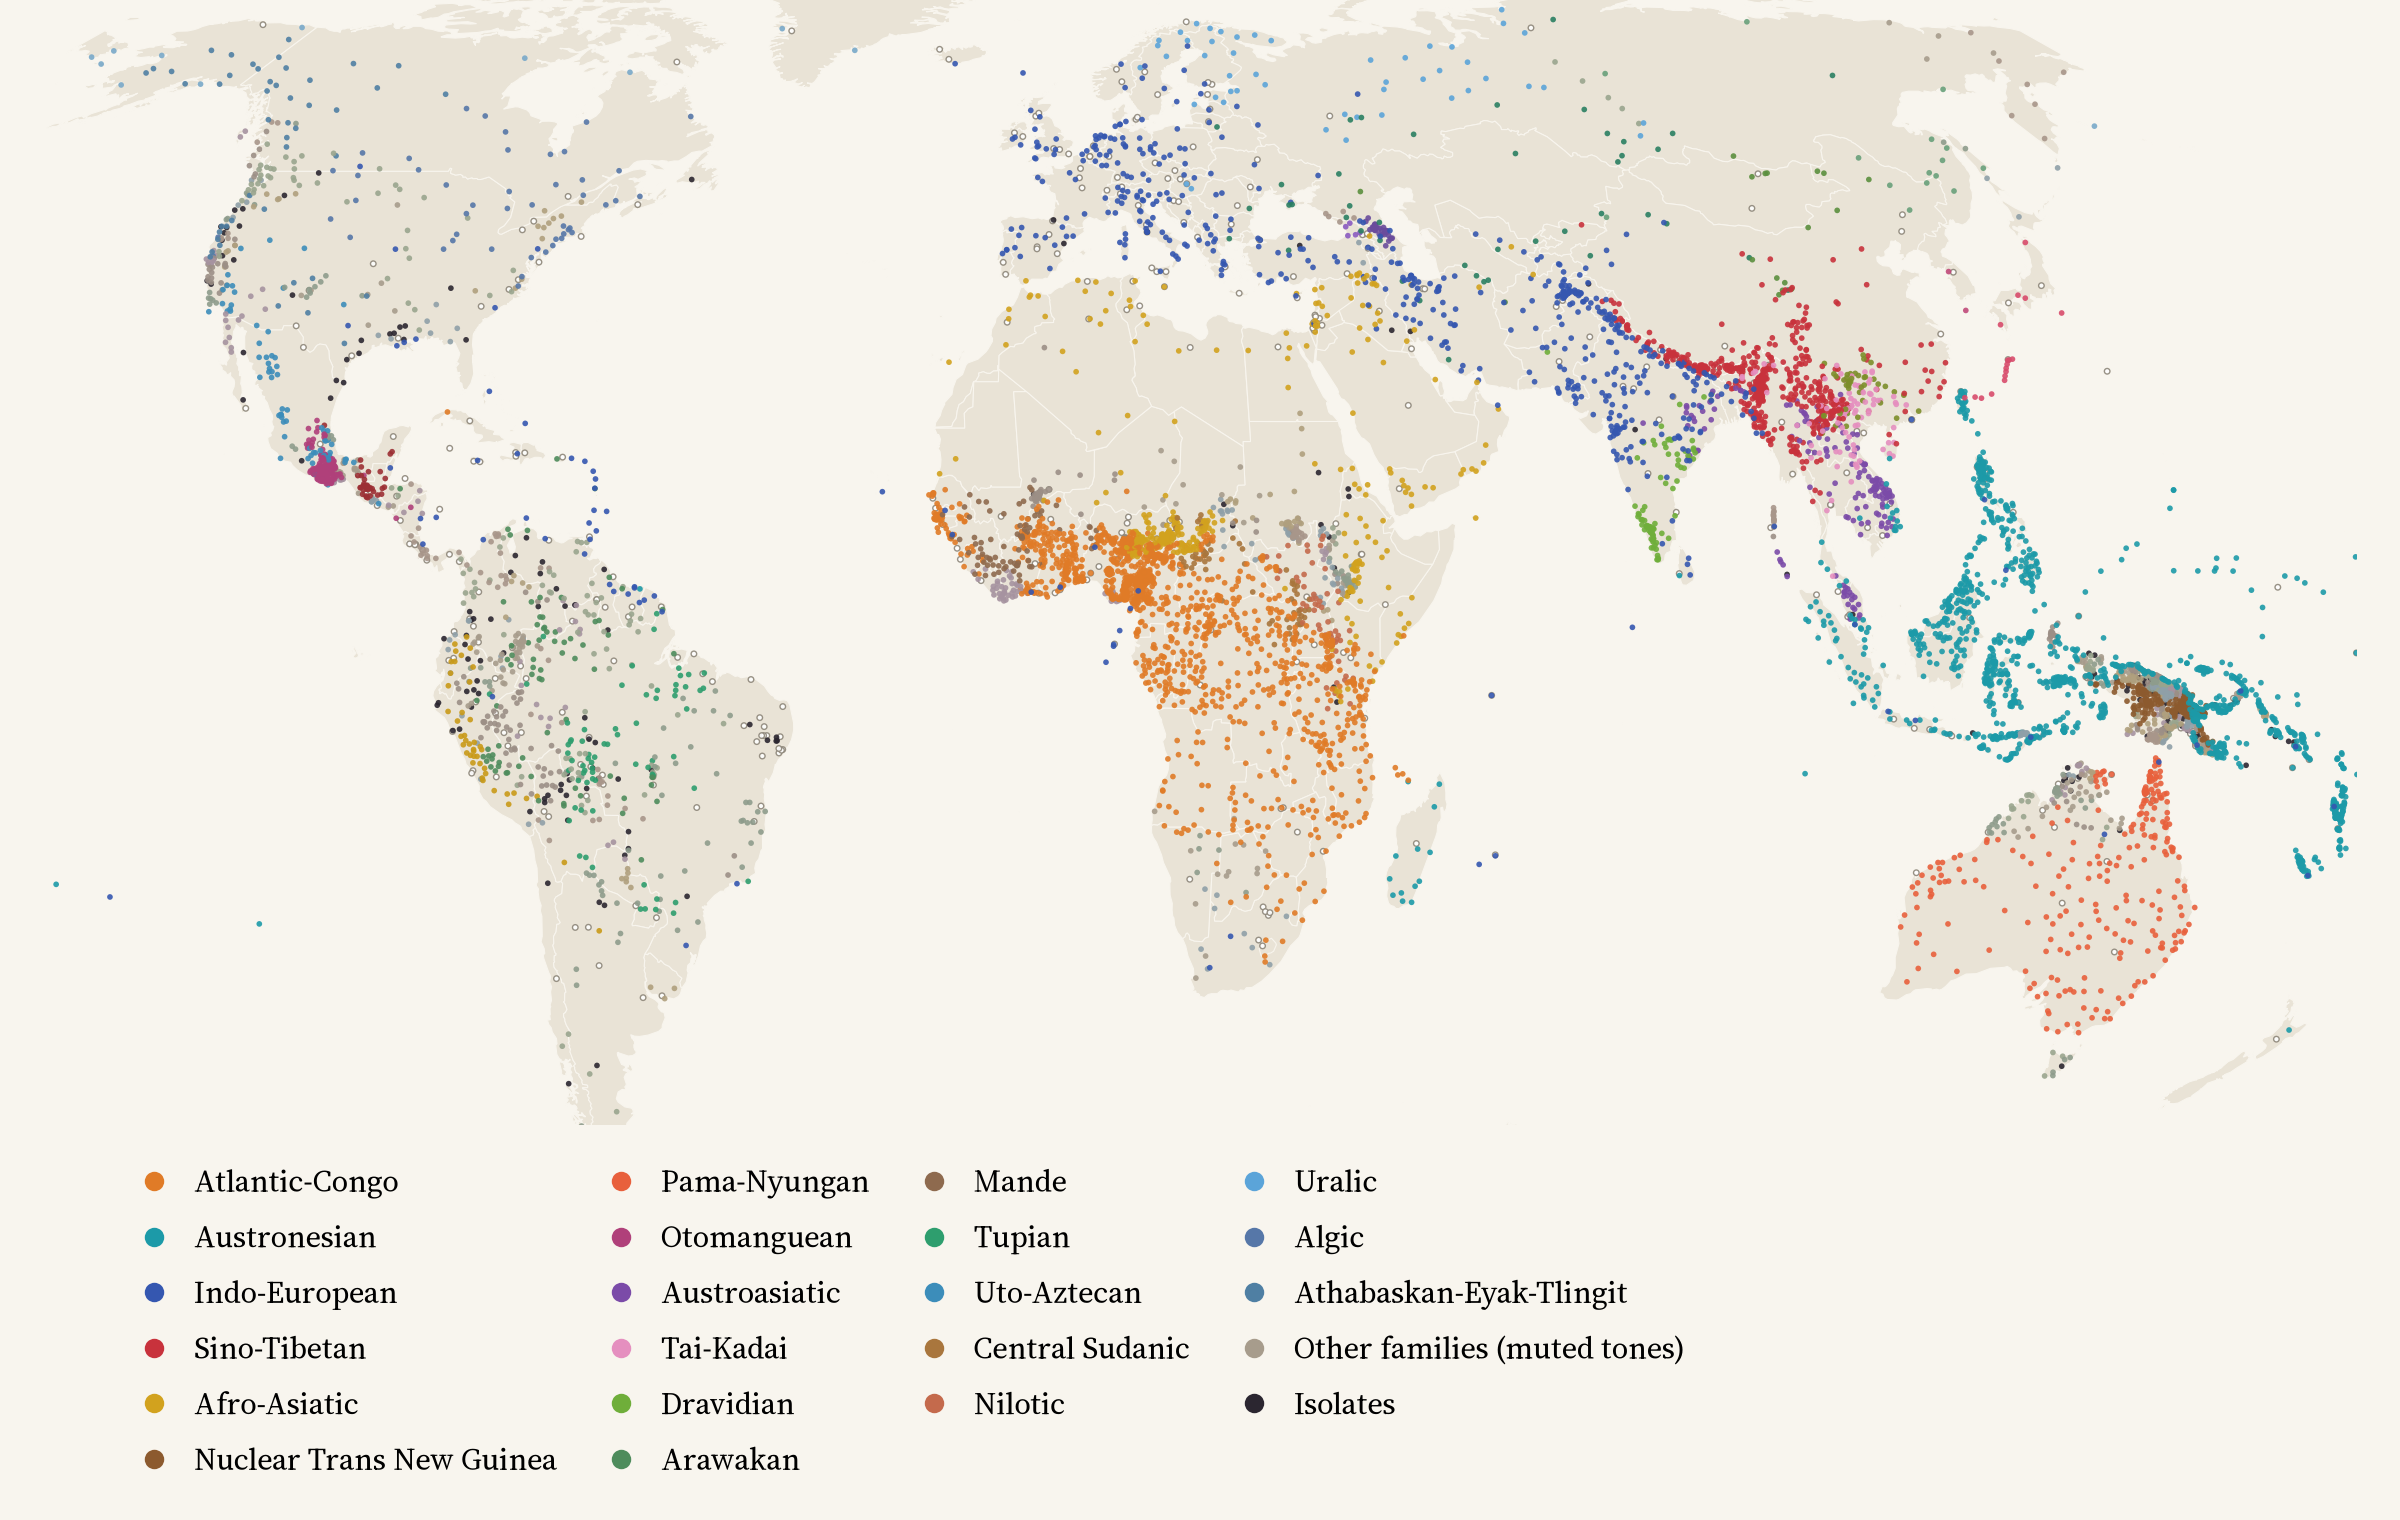
\includegraphics[width=\textwidth]{f_families_map.png}
\caption{Every spoken language in Glottolog 5.2.1 with a location, coloured by family. Isolates in black; sign languages, pidgins and other languages outside genealogical families as open circles. Equal Earth projection.}\label{fig:famap}\end{figure}

\begin{figure}[tbp]\centering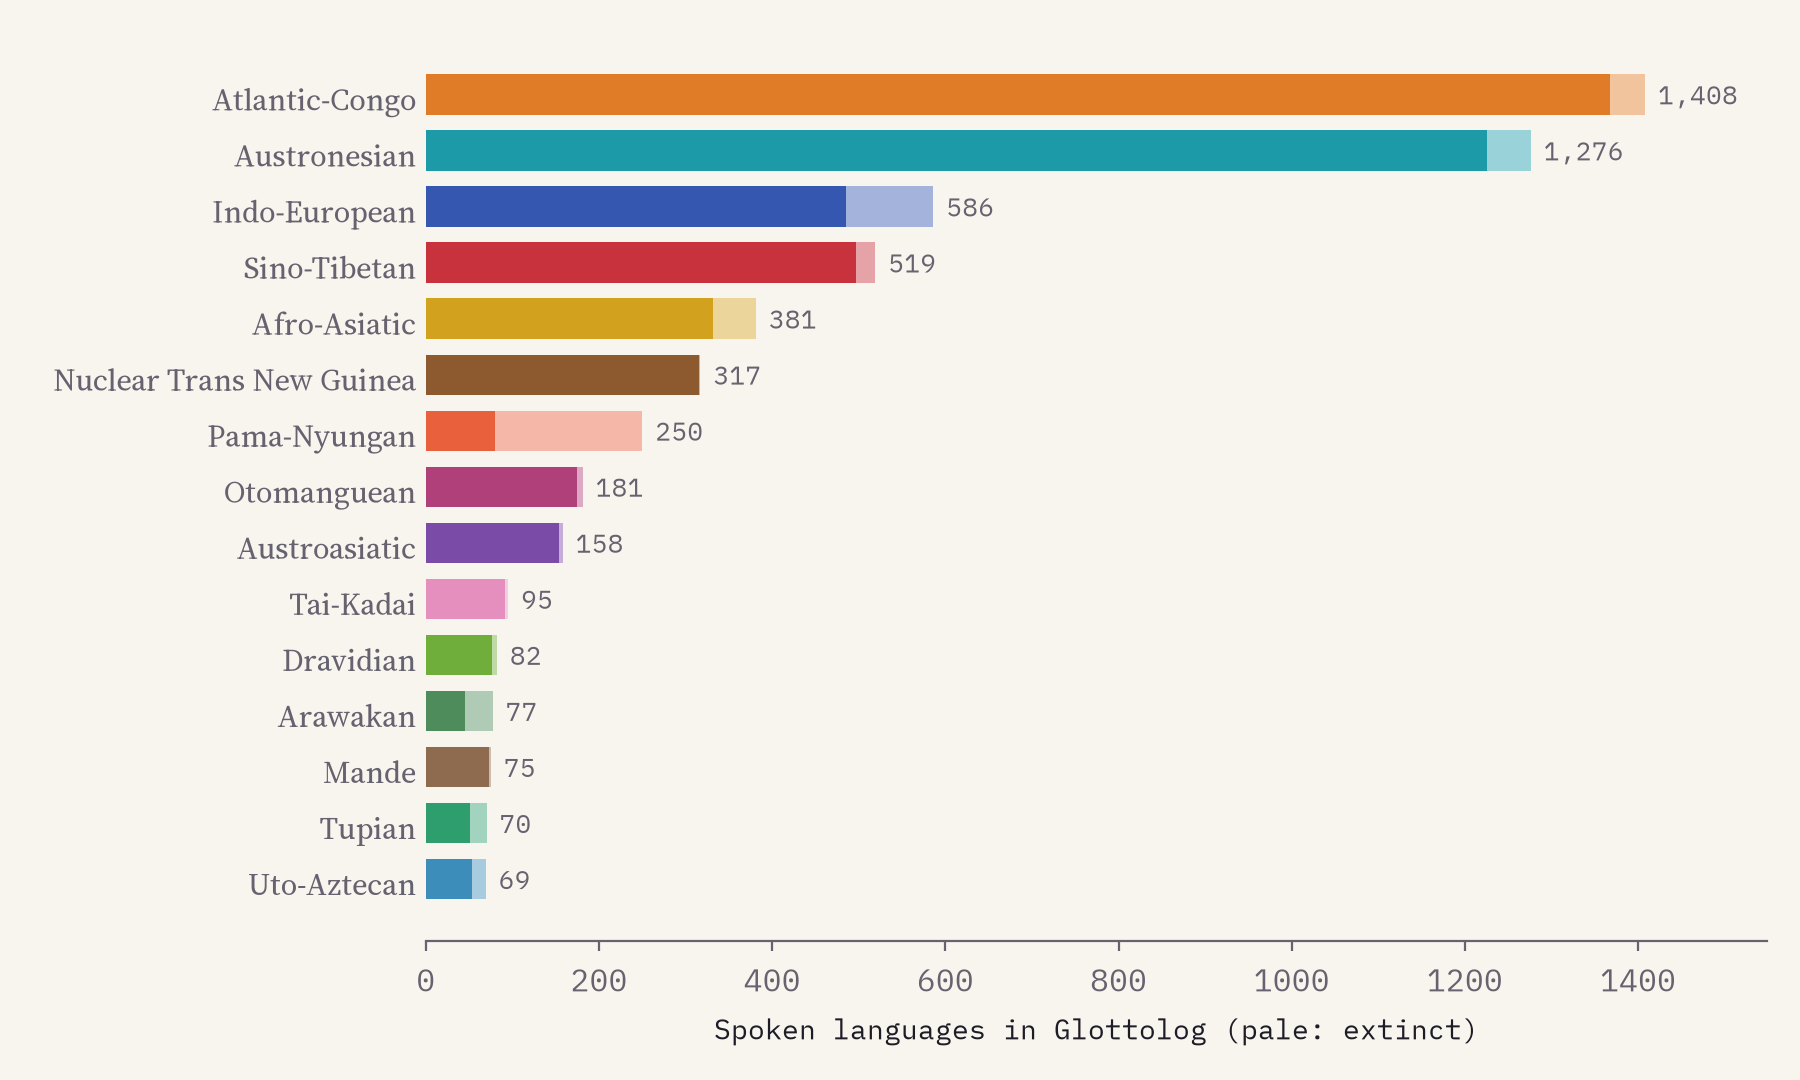
\includegraphics[width=.85\textwidth]{f_families.png}
\caption{The fifteen largest families by number of spoken languages; the pale part of each bar is extinct languages.}\label{fig:fams}\end{figure}

Selecting a family in the atlas colours it by its deep branches. Figure~\ref{fig:ie} shows Indo-European: Indo-Iranian alone has 321 languages, Germanic 106 and Italic 85, while Anatolian and Tokharian are known only from ancient texts.

\begin{figure}[tbp]\centering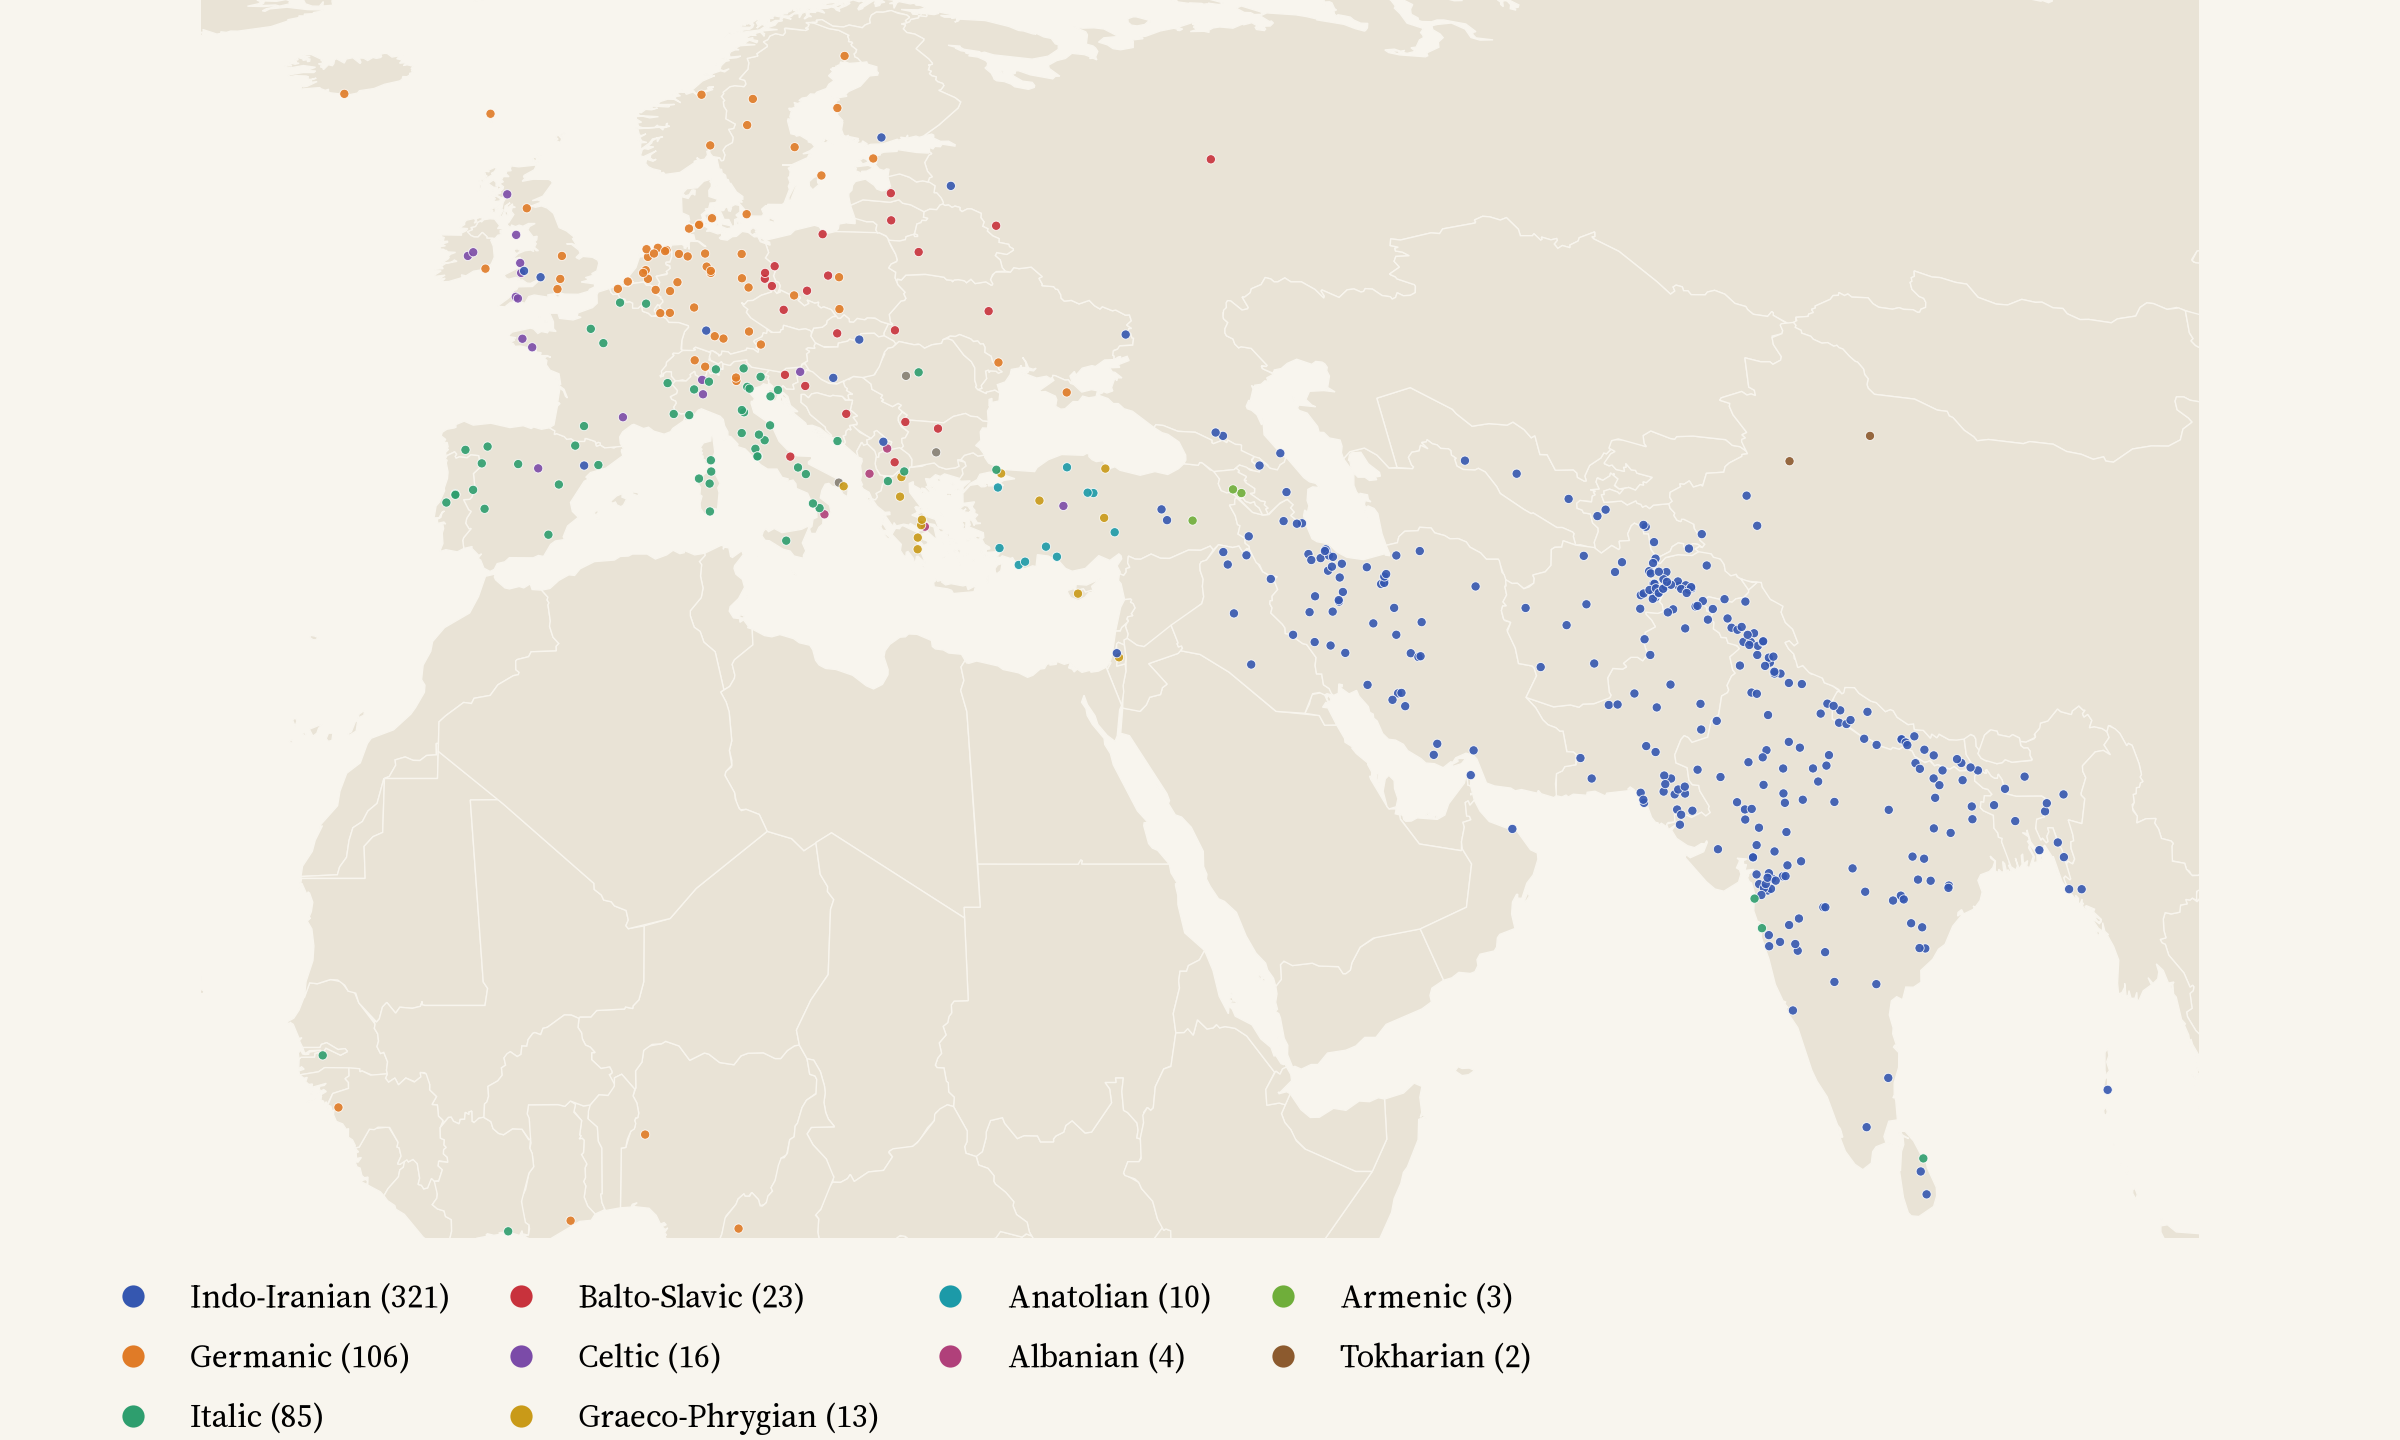
\includegraphics[width=\textwidth]{f_ie_branches.png}
\caption{Indo-European languages by deep branch (number of spoken languages in brackets, living and extinct).}\label{fig:ie}\end{figure}

\subsection{Where languages are concentrated}
Counting each living language in every country where it is spoken, Papua New Guinea has the most (850), followed by Indonesia (702), Nigeria (522), India (450) and China (395) (Figure~\ref{fig:cty}). Papua New Guinea also has the most lineages (77), ahead of Indonesia (55) and Brazil (31). Among countries of at least 10,000 km\textsuperscript{2}, Vanuatu has by far the highest density, 102.2 languages per 10,000 km\textsuperscript{2}, against 27.3 for the Solomon Islands and 18.4 for Papua New Guinea.

\begin{figure}[tbp]\centering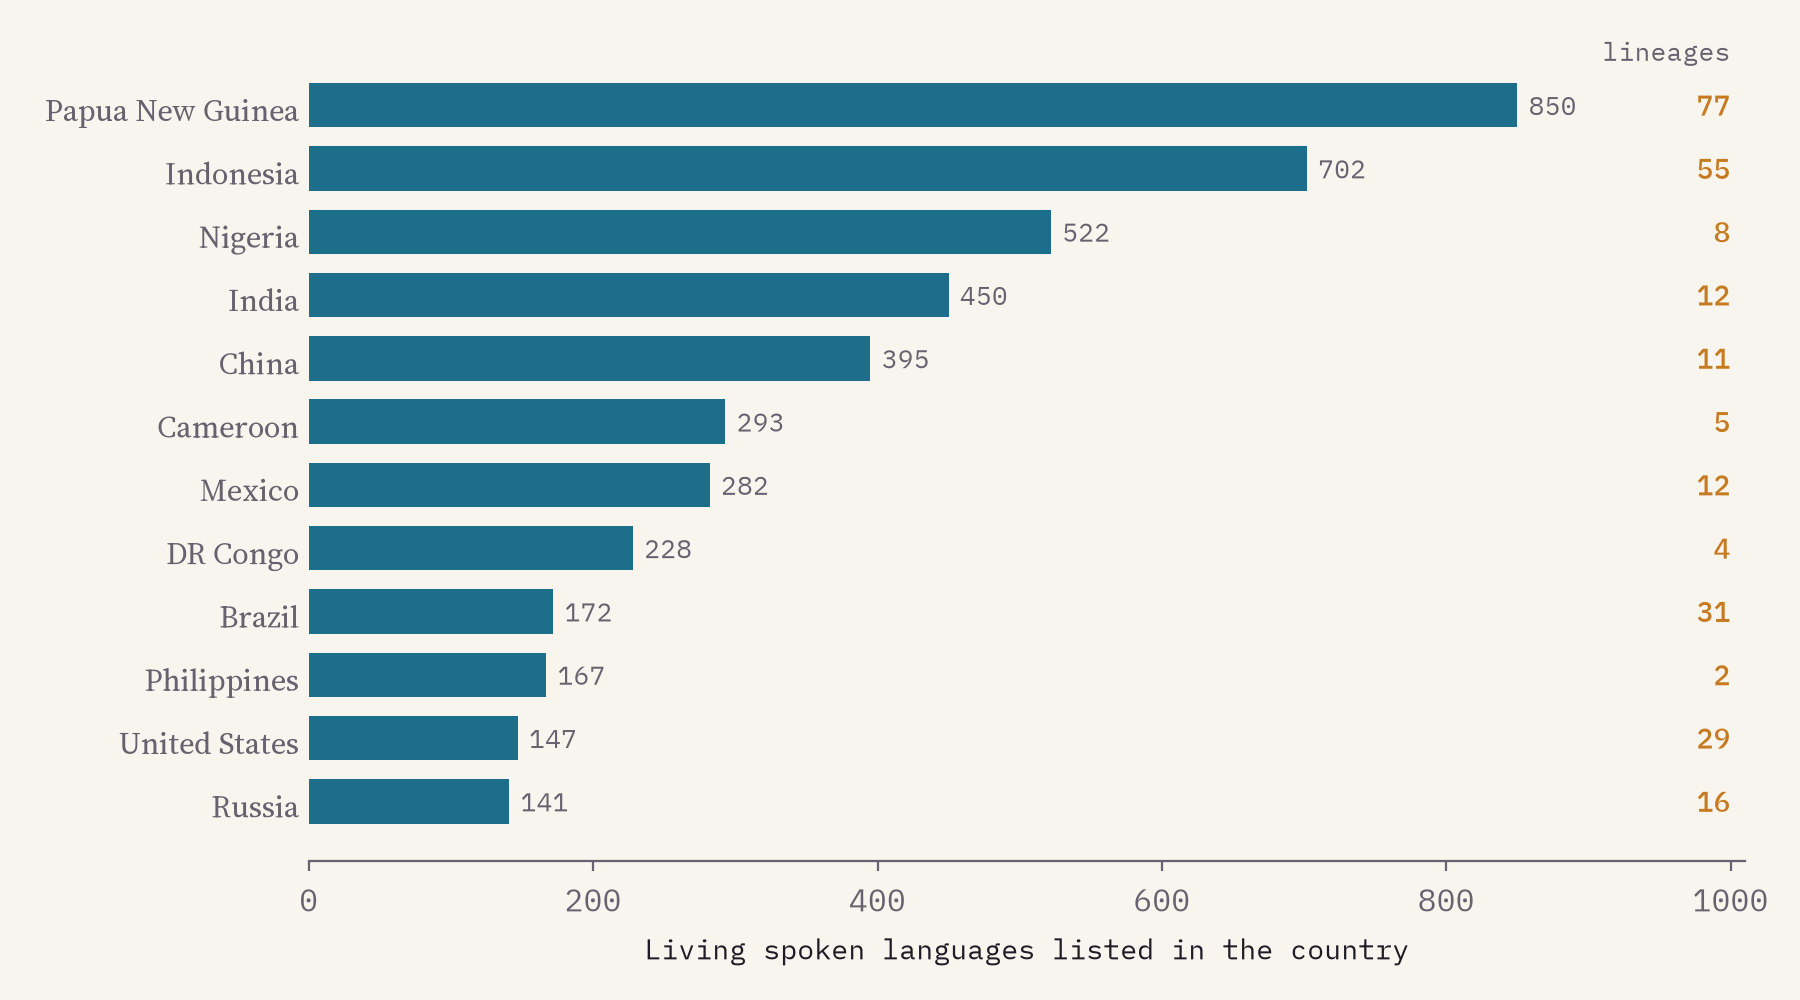
\includegraphics[width=.8\textwidth]{f_countries.png}
\caption{Countries with the most living spoken languages, with the number of lineages they belong to.}\label{fig:cty}\end{figure}

The equal-area grid shows the same concentration more sharply (Figure~\ref{fig:grid}, Table~\ref{tab:cells}). Of 4,510 land squares outside Antarctica, 1,627 contain at least one living language. The 45 densest (1\%) hold 27.6\% of the world's living languages and the densest 5\% hold 59.0\%. The single densest square, in Madang, Papua New Guinea, contains 148 living languages; the square with most lineages, in Sandaun, Papua New Guinea, contains 23. The densest squares form a tropical belt through New Guinea and Melanesia, the Nigeria and Cameroon borderland, southern Mexico and the eastern Himalaya.

\begin{figure}[tbp]\centering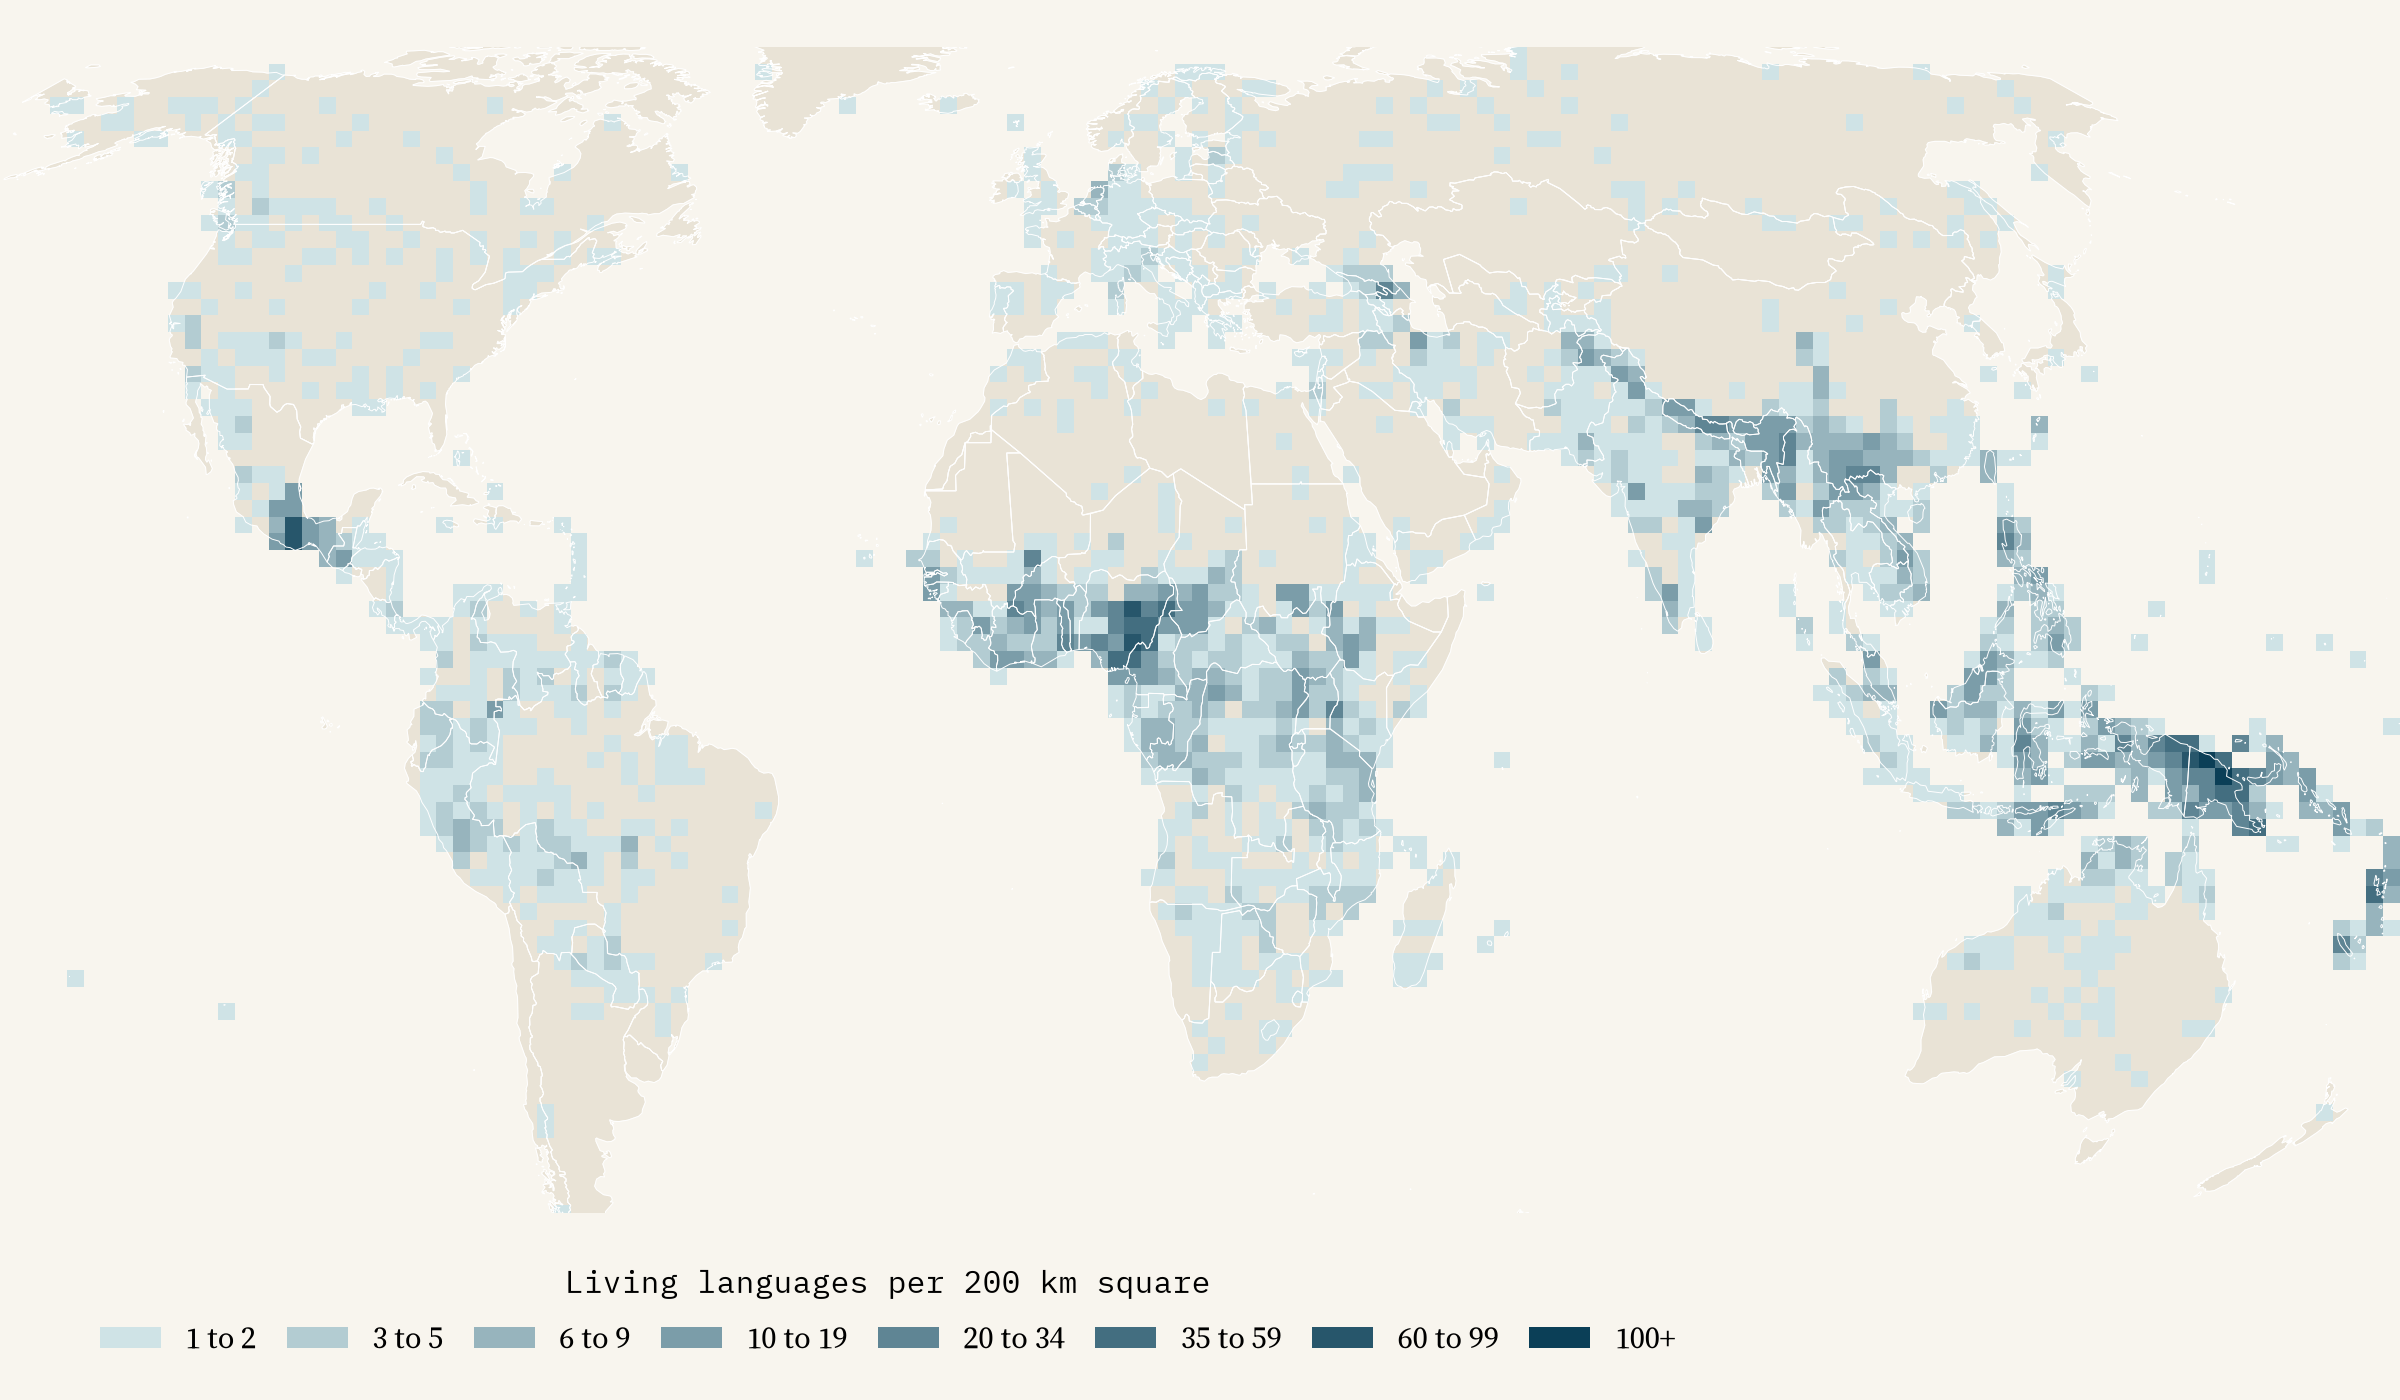
\includegraphics[width=\textwidth]{f_diversity_map.png}
\caption{Living spoken languages per 200 by 200 km square of the Equal Earth projection.}\label{fig:grid}\end{figure}

\begin{table}[tbp]\centering\small\caption{The eight 200 km squares with the most living languages, named by the admin-1 region where most of their languages lie.}\label{tab:cells}\begin{tabular}{lrr}\toprule Square (region, country) & Living languages & Lineages\\\midrule
Madang, Papua New Guinea & 148 & 4\\
East Sepik, Papua New Guinea & 105 & 9\\
Oaxaca, Mexico & 80 & 2\\
Bauchi, Nigeria & 68 & 2\\
Sandaun, Papua New Guinea & 65 & 23\\
Oaxaca, Mexico & 64 & 3\\
Nord-Ouest, Cameroon & 61 & 1\\
Nord-Ouest, Cameroon & 57 & 2\\
\bottomrule\end{tabular}\end{table}

\subsection{Endangerment}
Only 35.0\% of spoken languages are rated not endangered (Figure~\ref{fig:aes}). 20.1\% are threatened, 22.8\% shifting, 5.4\% moribund and 3.8\% nearly extinct: 3,998 endangered languages, 52.1\% of all and 59.7\% of those still spoken. 981 (12.8\%) are extinct. The regional pattern follows the history of colonial settlement: 63.9\% of languages in Glottolog's Australia macroarea are extinct, 35.1\% in South America and 28.2\% in North America, against 11.8\% in Eurasia, 4.2\% in Africa and 3.1\% in Papunesia. Africa has the largest share rated not endangered (58.9\%). Of the 421 lineages, 324 (77.0\%) have no language rated not endangered, and 98 of the 103 living isolates are endangered. Documentation is thin as well: for 61.8\% of spoken languages the most extensive description is less than a grammar, and for 18.7\% it is a word list or less.

\begin{figure}[tbp]\centering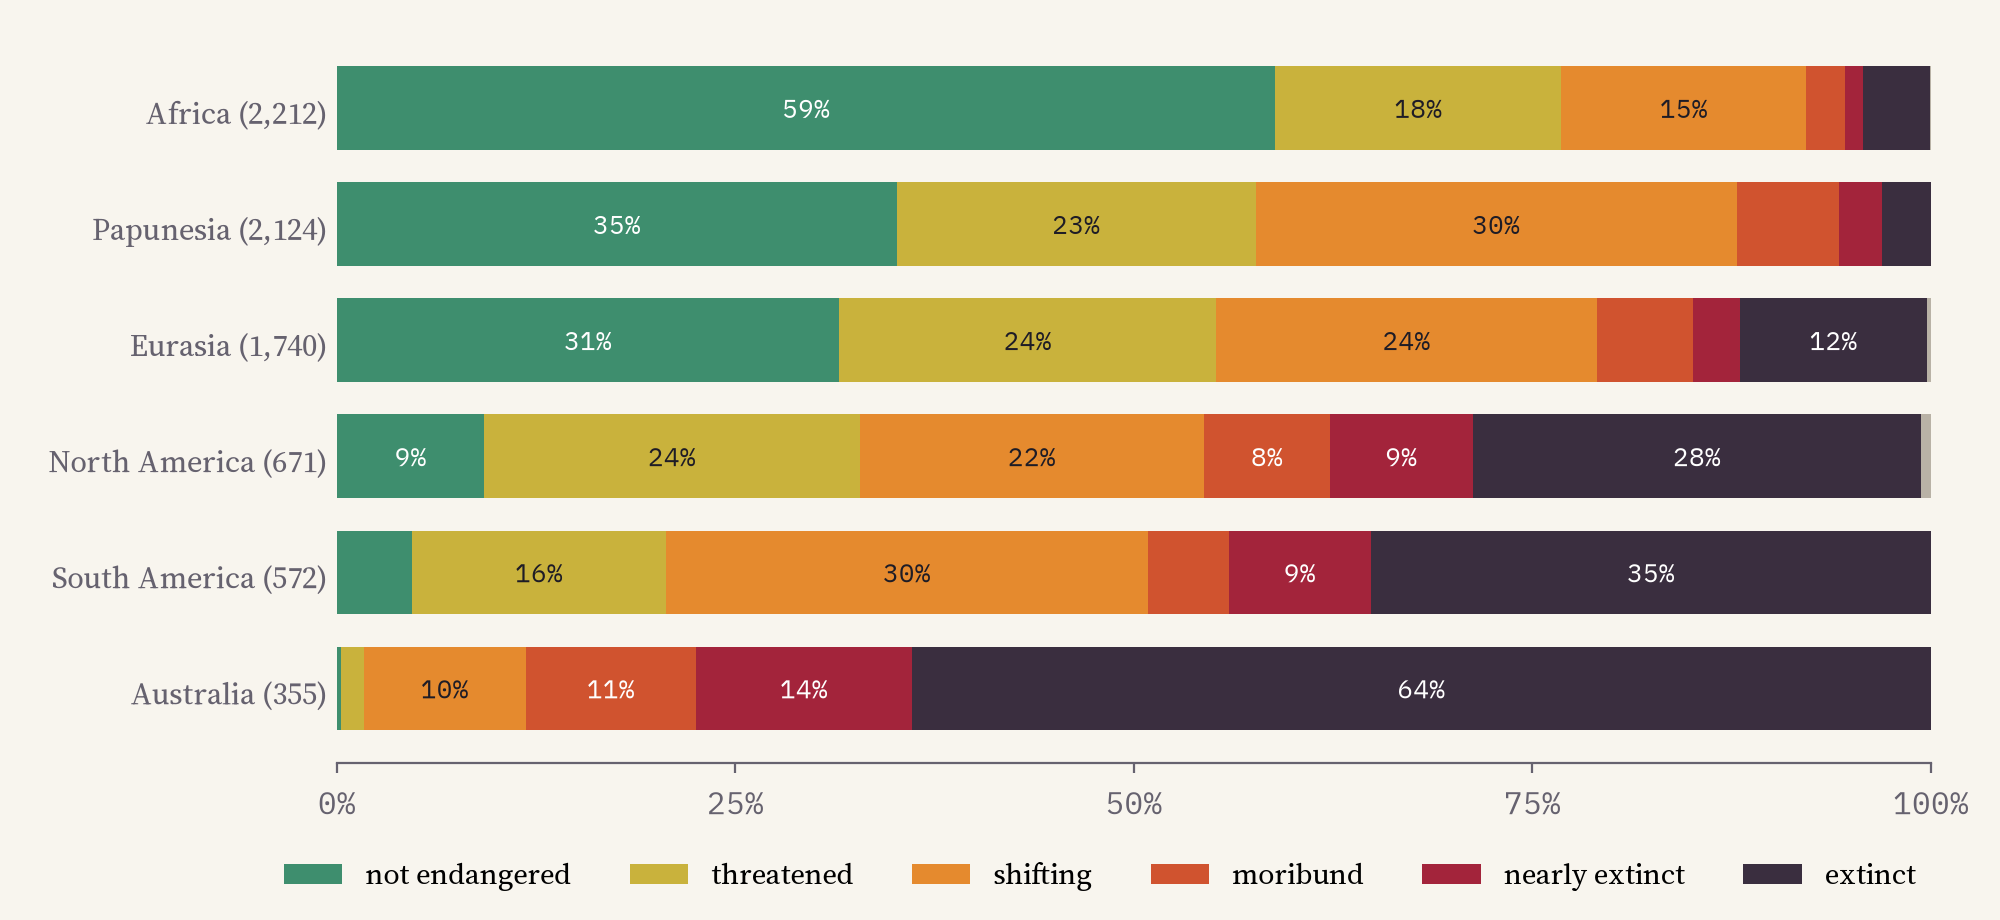
\includegraphics[width=.92\textwidth]{f_aes_macro.png}
\caption{Agglomerated Endangerment Status of spoken languages by Glottolog macroarea (number of languages in brackets).}\label{fig:aes}\end{figure}

\begin{figure}[tbp]\centering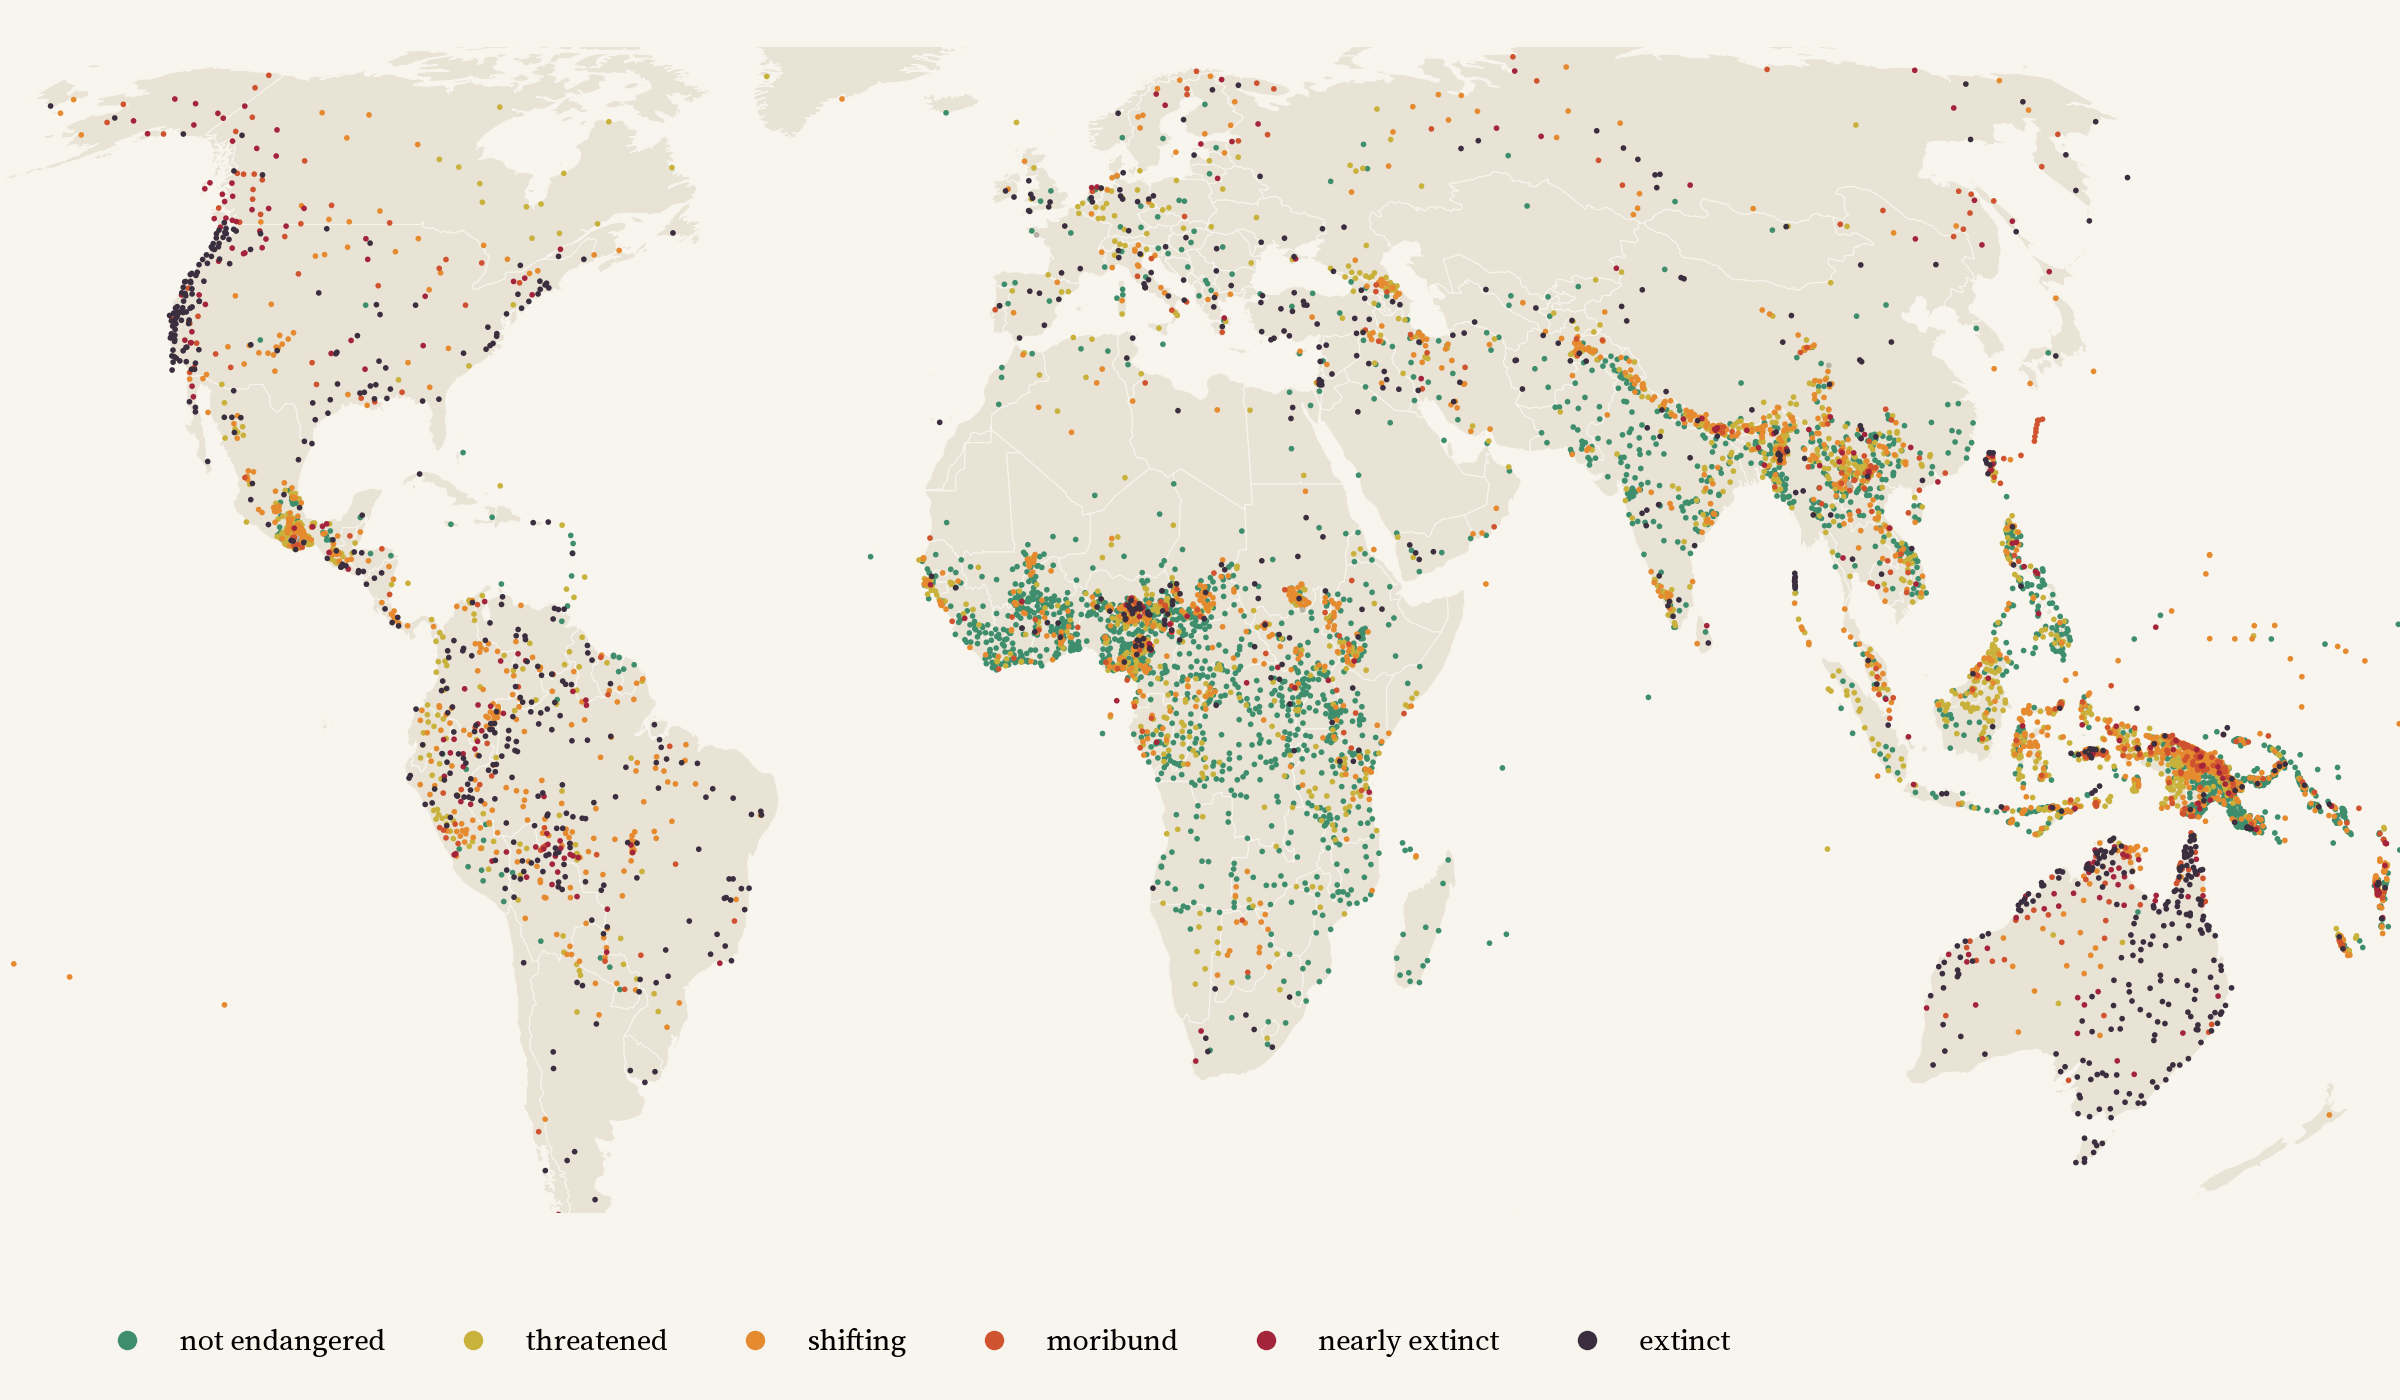
\includegraphics[width=\textwidth]{f_aes_map.png}
\caption{Spoken languages by Agglomerated Endangerment Status; more endangered languages are drawn on top.}\label{fig:aesmap}\end{figure}

\subsection{Speakers}
The Wikidata counts cover 1,627 of the 7,674 spoken languages (21.2\%, or 24.3\% of living languages), and they are biased towards larger languages: 37.9\% of languages with a count are rated not endangered, against 35.0\% of all. They add up to 6.9 billion, a figure that mixes first-language and total counts and years and should not be read as a census. The concentration is nevertheless striking (Figure~\ref{fig:sp}). The 10 largest languages account for 50.9\% of all speakers counted, the 20 largest for 62.6\% and the 100 largest for 89.8\%; half of all counted speakers speak one of just 10 languages, 0.13\% of the world's spoken languages. The median language with a count has 20,000 speakers; 374 have fewer than 1,000. Indo-European languages account for 45.4\% of counted speakers and Sino-Tibetan for 19.6\%.

\begin{figure}[tbp]\centering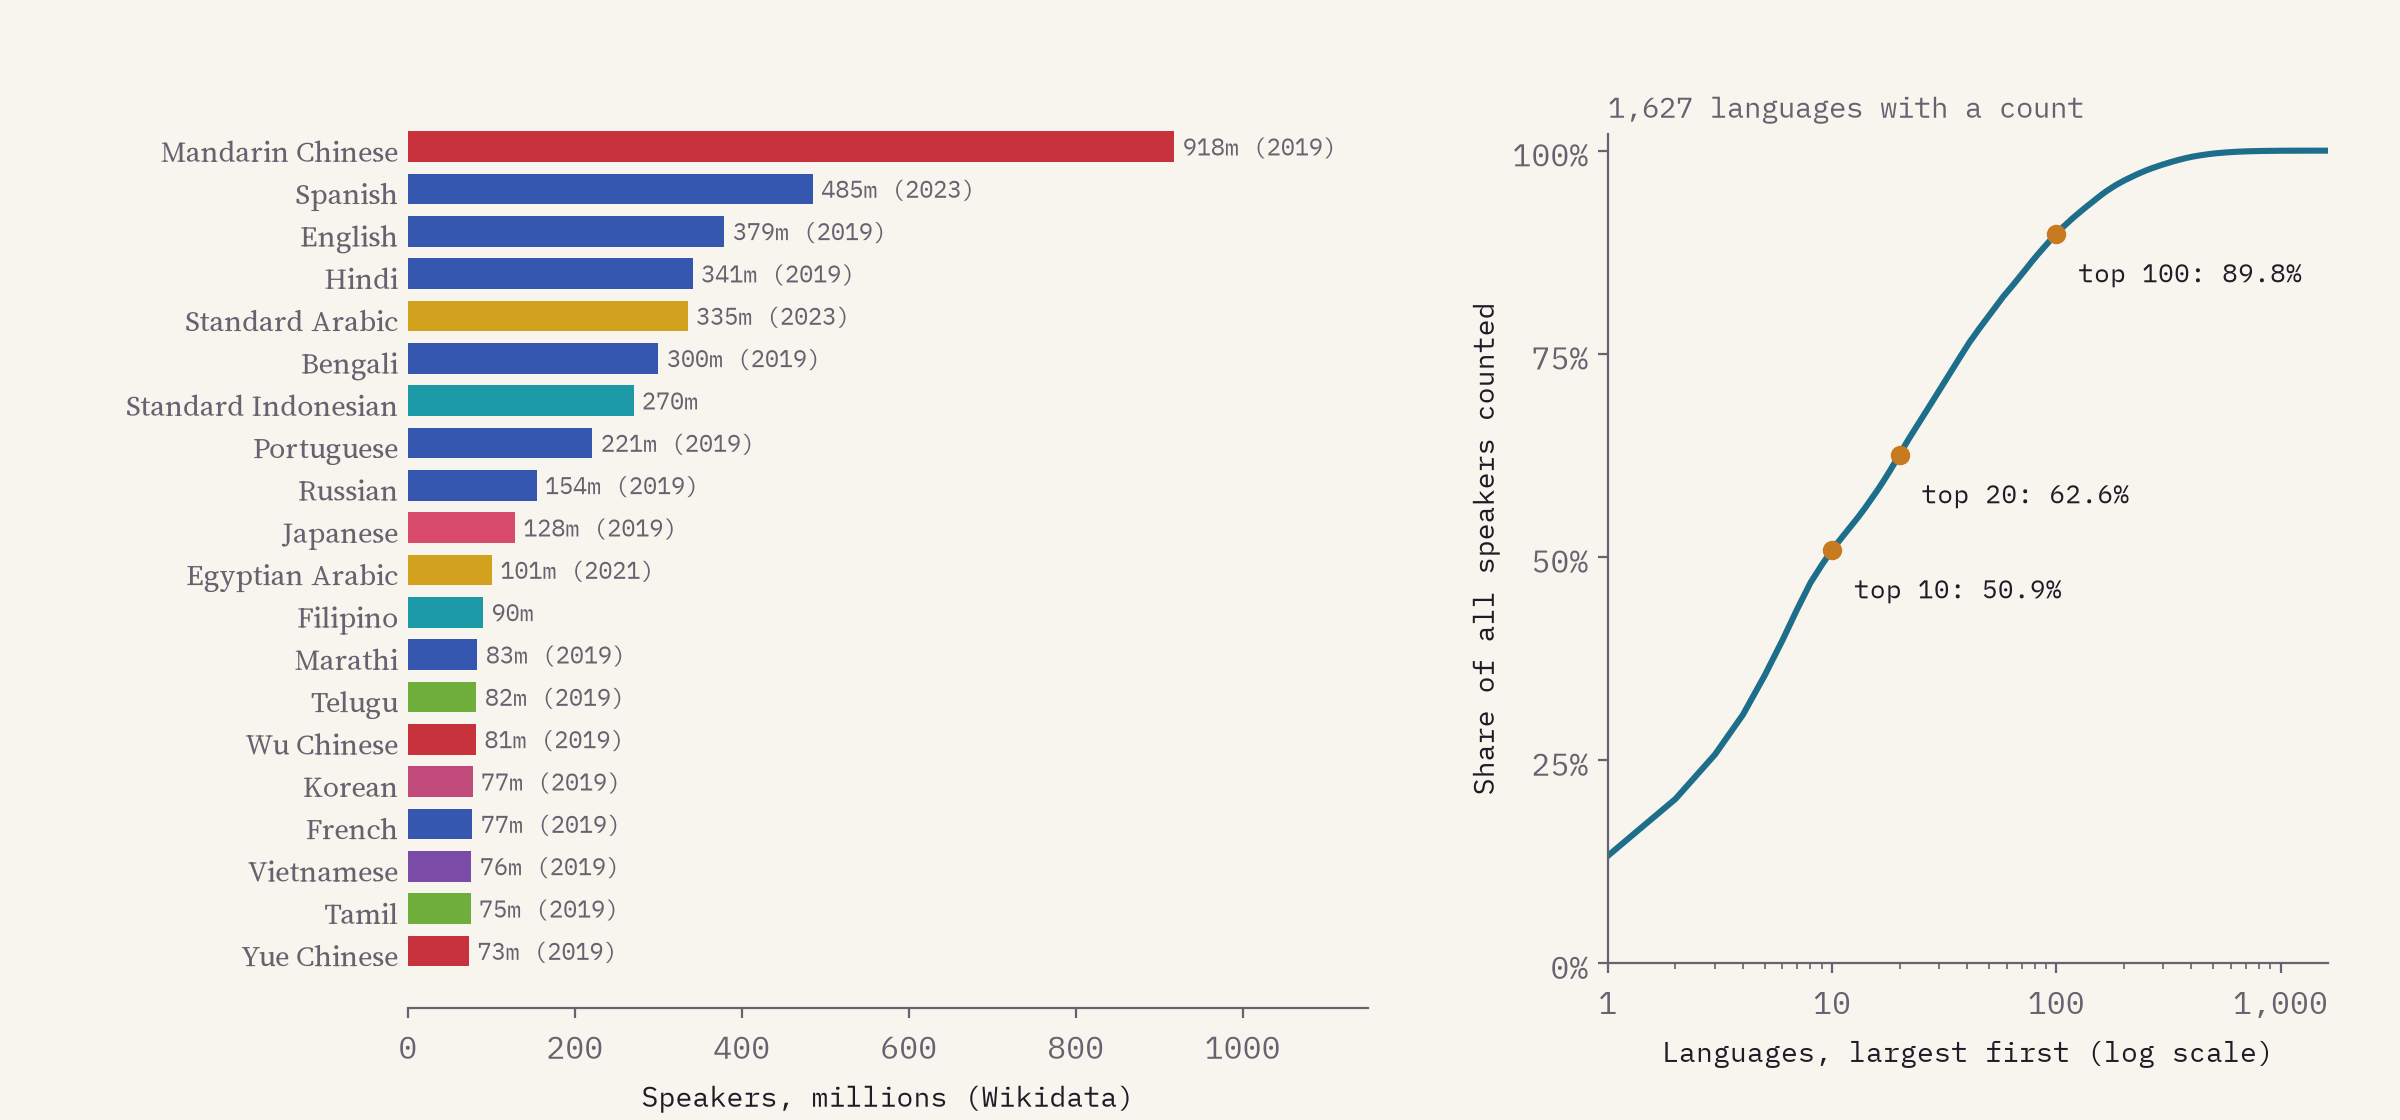
\includegraphics[width=\textwidth]{f_speakers.png}
\caption{Left: the 20 largest languages by Wikidata speaker count (millions, year of the count in brackets), coloured by family. Right: cumulative share of all speakers counted, languages ranked from largest.}\label{fig:sp}\end{figure}

\subsection{Origins}
Table~\ref{tab:homelands} lists the 16 homeland hypotheses for 11 families, and Figure~\ref{fig:orig} maps them with the computed centres. Figure~\ref{fig:dist} gives the distances.

{\small\setlength{\tabcolsep}{4pt}\begin{longtable}{>{\raggedright\arraybackslash}p{2.1cm}>{\raggedright\arraybackslash}p{5.1cm}>{\raggedright\arraybackslash}p{4.1cm}>{\raggedright\arraybackslash}p{3.6cm}}\caption{Proposed homelands and dates from the literature. Places are approximate centres of the proposed regions. These are hypotheses, several of them contested.}\label{tab:homelands}\\\toprule Family & Hypothesis and place & When & Sources\\\midrule\endfirsthead\toprule Family & Hypothesis and place & When & Sources\\\midrule\endhead
Indo-European & \textbf{Steppe hypothesis}: Pontic-Caspian steppe, north of the Black and Caspian seas & roughly 4,500 to 6,500 years ago (Anthony's c. 4500 to 2500 BCE) & \citealt{anthony2007}; \citealt{anthony2015}; \citealt{haak2015}\\
Indo-European & \textbf{Anatolian hypothesis}: Central Anatolia (modern Turkey) & roughly 8,000 to 9,500 years ago, with the spread of farming (the authors' approximate range) & \citealt{renfrew1987}; \citealt{bouckaert2012}\\
Indo-European & \textbf{Hybrid hypothesis}: South of the Caucasus (northern Fertile Crescent) & about 8,100 years ago for the first split (the authors' estimate) & \citealt{heggarty2023}\\
Austronesian & \textbf{Out of Taiwan}: Taiwan & roughly 5,000 to 5,500 years ago & \citealt{blust1999}; \citealt{gray2009}\\
Bantu & \textbf{Grassfields origin}: Cameroon and Nigeria borderland (Grassfields) & roughly 4,000 to 5,000 years ago & \citealt{vansina1995}; \citealt{grollemund2015}\\
Uralic & \textbf{Volga-Kama}: Middle Volga, Kama and the Ural Mountains (approximate) & no single agreed date; a dated phylogeny puts the family's first splits several thousand years ago & \citealt{honkola2013}\\
Uralic & \textbf{Western Siberia}: Western Siberia, the Sayan and upper Yenisei area (approximate) & spread west from about 4,200 years ago & \citealt{grunthal2022}; \citealt{janhunen2009}\\
Turkic & \textbf{Eastern steppe}: Mongolia and southern Siberia & about 2,100 years ago for the first split, Bolgar and Common Turkic (95\% range 1,500 to 2,800) & \citealt{golden1992}; \citealt{savelyev2020}\\
Sino-Tibetan & \textbf{Yellow River}: Upper and middle Yellow River basin, northern China & roughly 5,900 to 7,200 years ago (the two studies' estimates) & \citealt{zhang2019}; \citealt{sagart2019}\\
Afro-Asiatic & \textbf{African origin}: Horn of Africa and the Red Sea hills & more than 10,000 years ago, by Ehret's reckoning possibly much earlier & \citealt{ehret1995}; \citealt{ehret2004}\\
Afro-Asiatic & \textbf{Levantine origin}: The Levant & more than 10,000 years ago, linked by Militarev to the Natufian & \citealt{militarev2002}\\
Niger-Congo & \textbf{West African origin}: West Africa, perhaps the inland Niger region & probably more than 10,000 years ago; no agreed date & \citealt{williamson2000}; \citealt{guldemann2018}\\
Pama-Nyungan & \textbf{Gulf Plains}: Gulf Plains of north-west Queensland, Australia & roughly 6,000 years ago (the authors' approximate estimate) & \citealt{bouckaert2018}\\
Uto-Aztecan & \textbf{Southern origin}: Northern and central Mexico & roughly 4,000 to 5,000 years ago & \citealt{hill2001}\\
Uto-Aztecan & \textbf{Northern origin}: South-western United States, southern Great Basin & roughly 4,000 to 5,000 years ago & \citealt{fowler1983}\\
Quechuan & \textbf{Central Peru}: Central coast and highlands of Peru & roughly 1,500 to 2,500 years ago & \citealt{torero1964}; \citealt{adelaar2004}\\
\bottomrule\end{longtable}}

\begin{figure}[tbp]\centering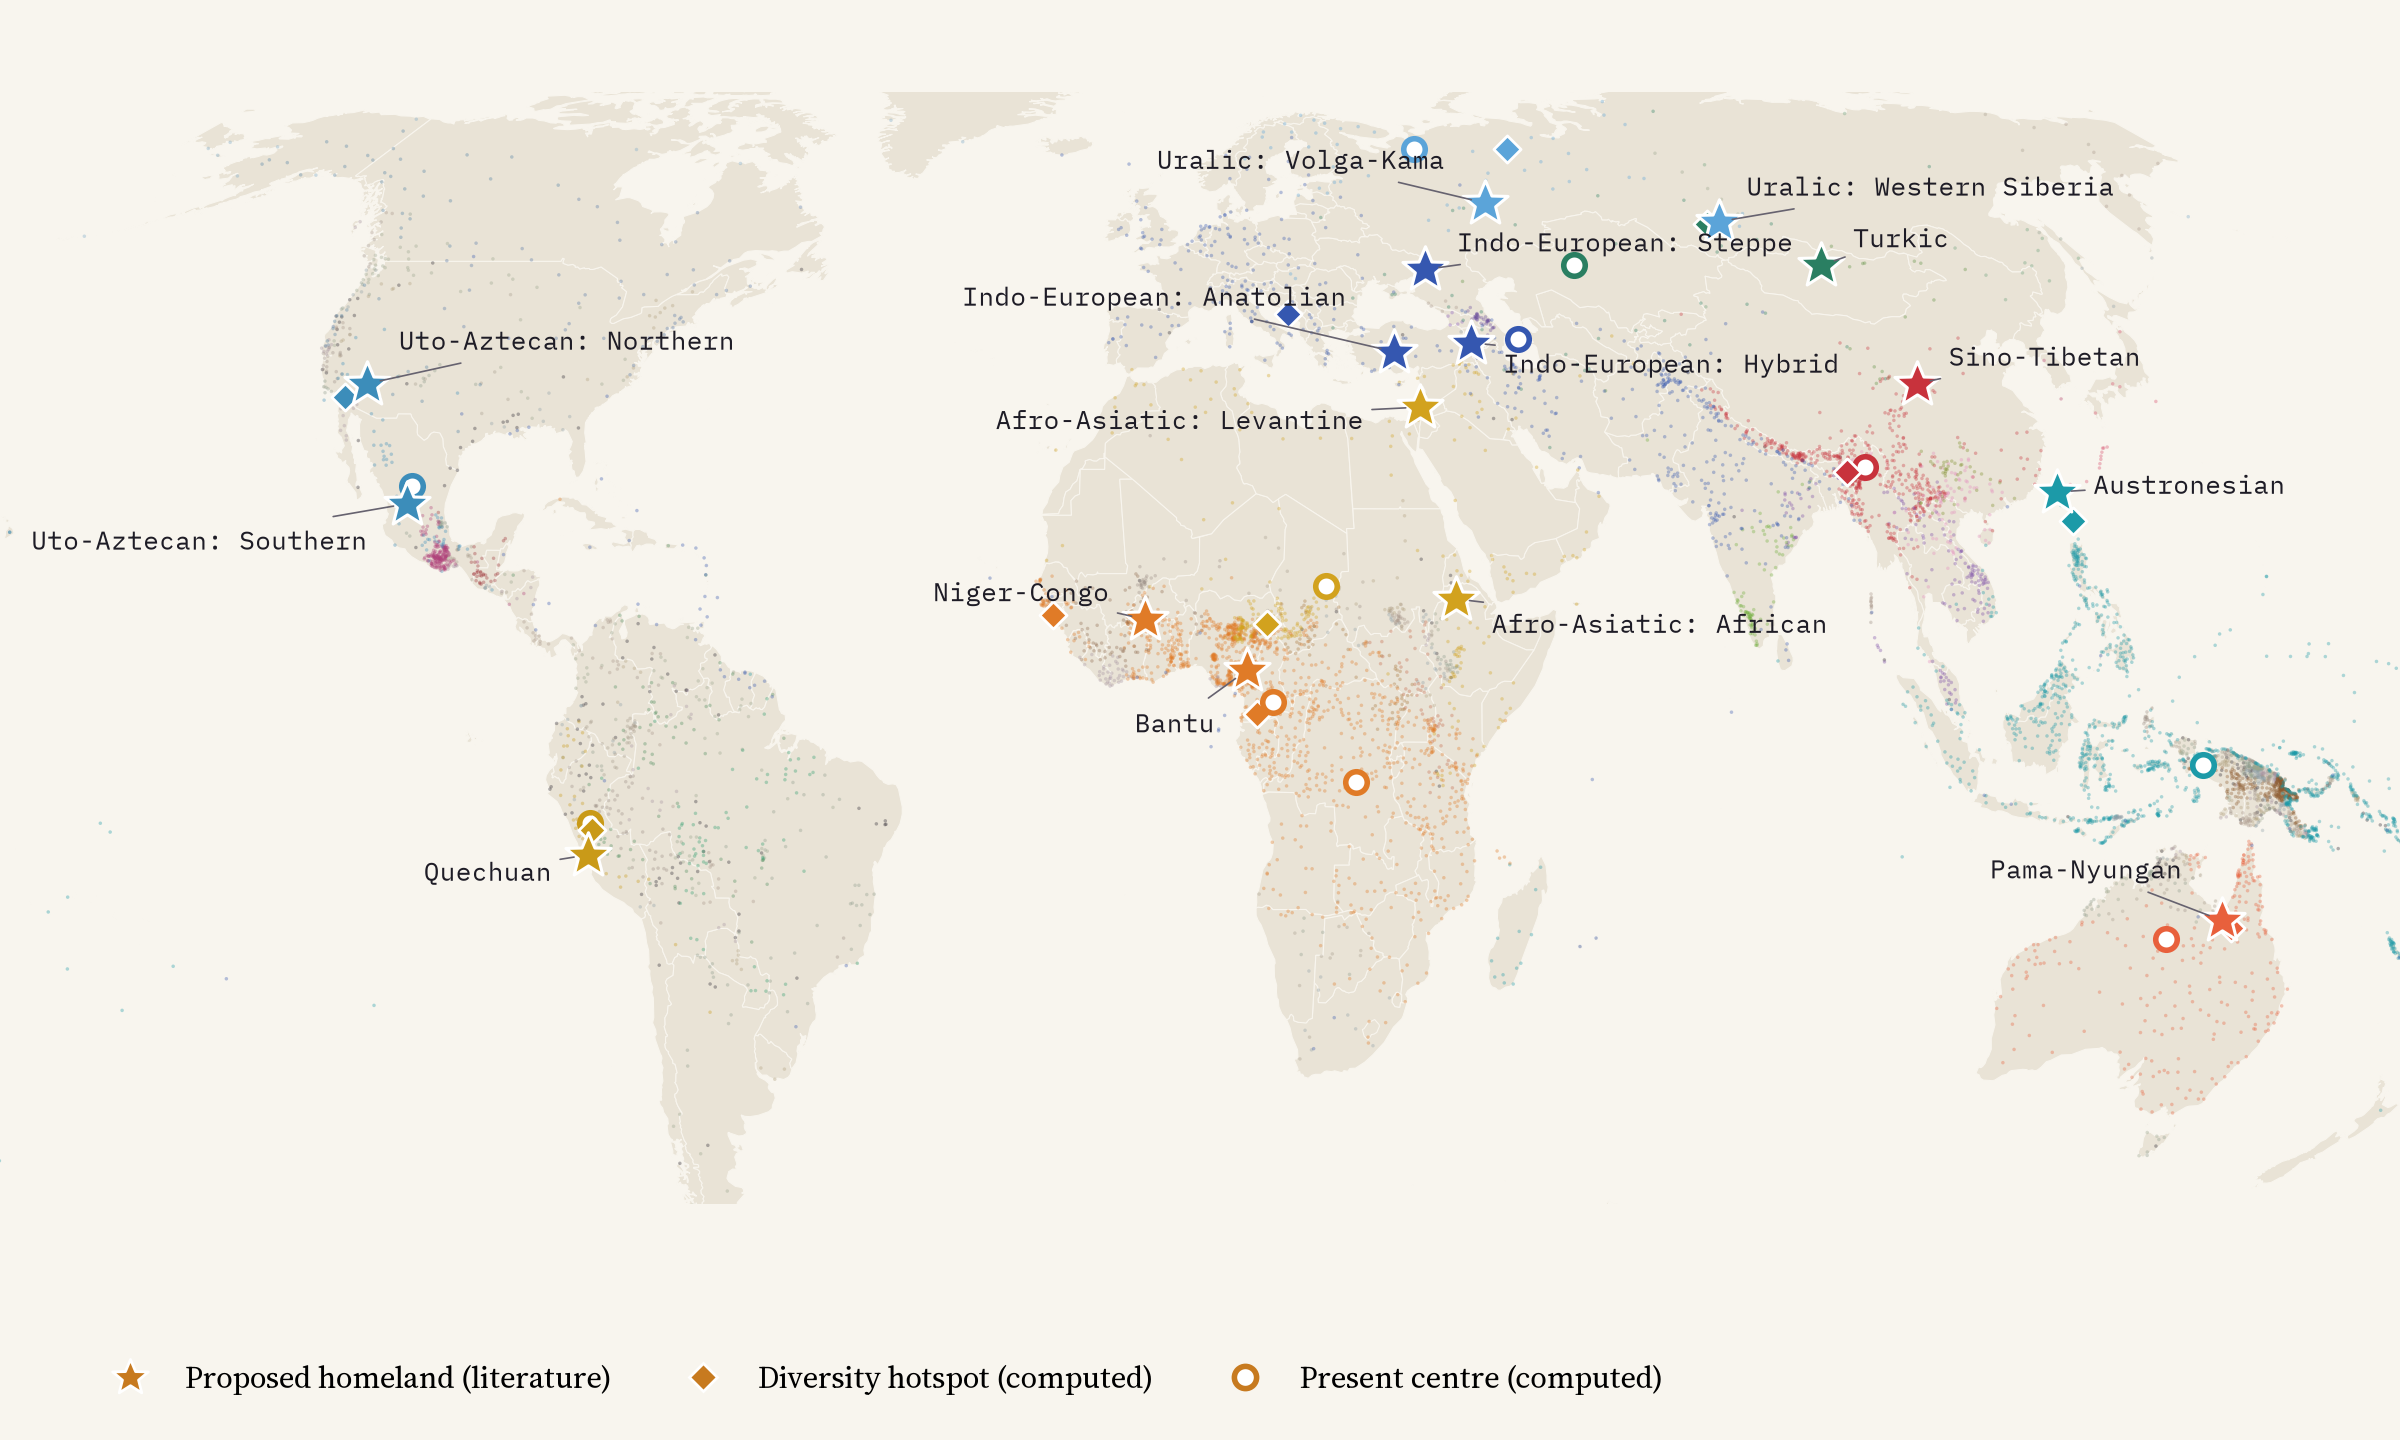
\includegraphics[width=\textwidth]{f_origins_map.png}
\caption{Proposed homelands from the literature (stars), with each family's diversity hotspot (diamonds) and present centre (rings) computed from Glottolog. Faint dots are all languages, coloured by family. Niger-Congo's computed points are for Atlantic-Congo.}\label{fig:orig}\end{figure}

\begin{figure}[tbp]\centering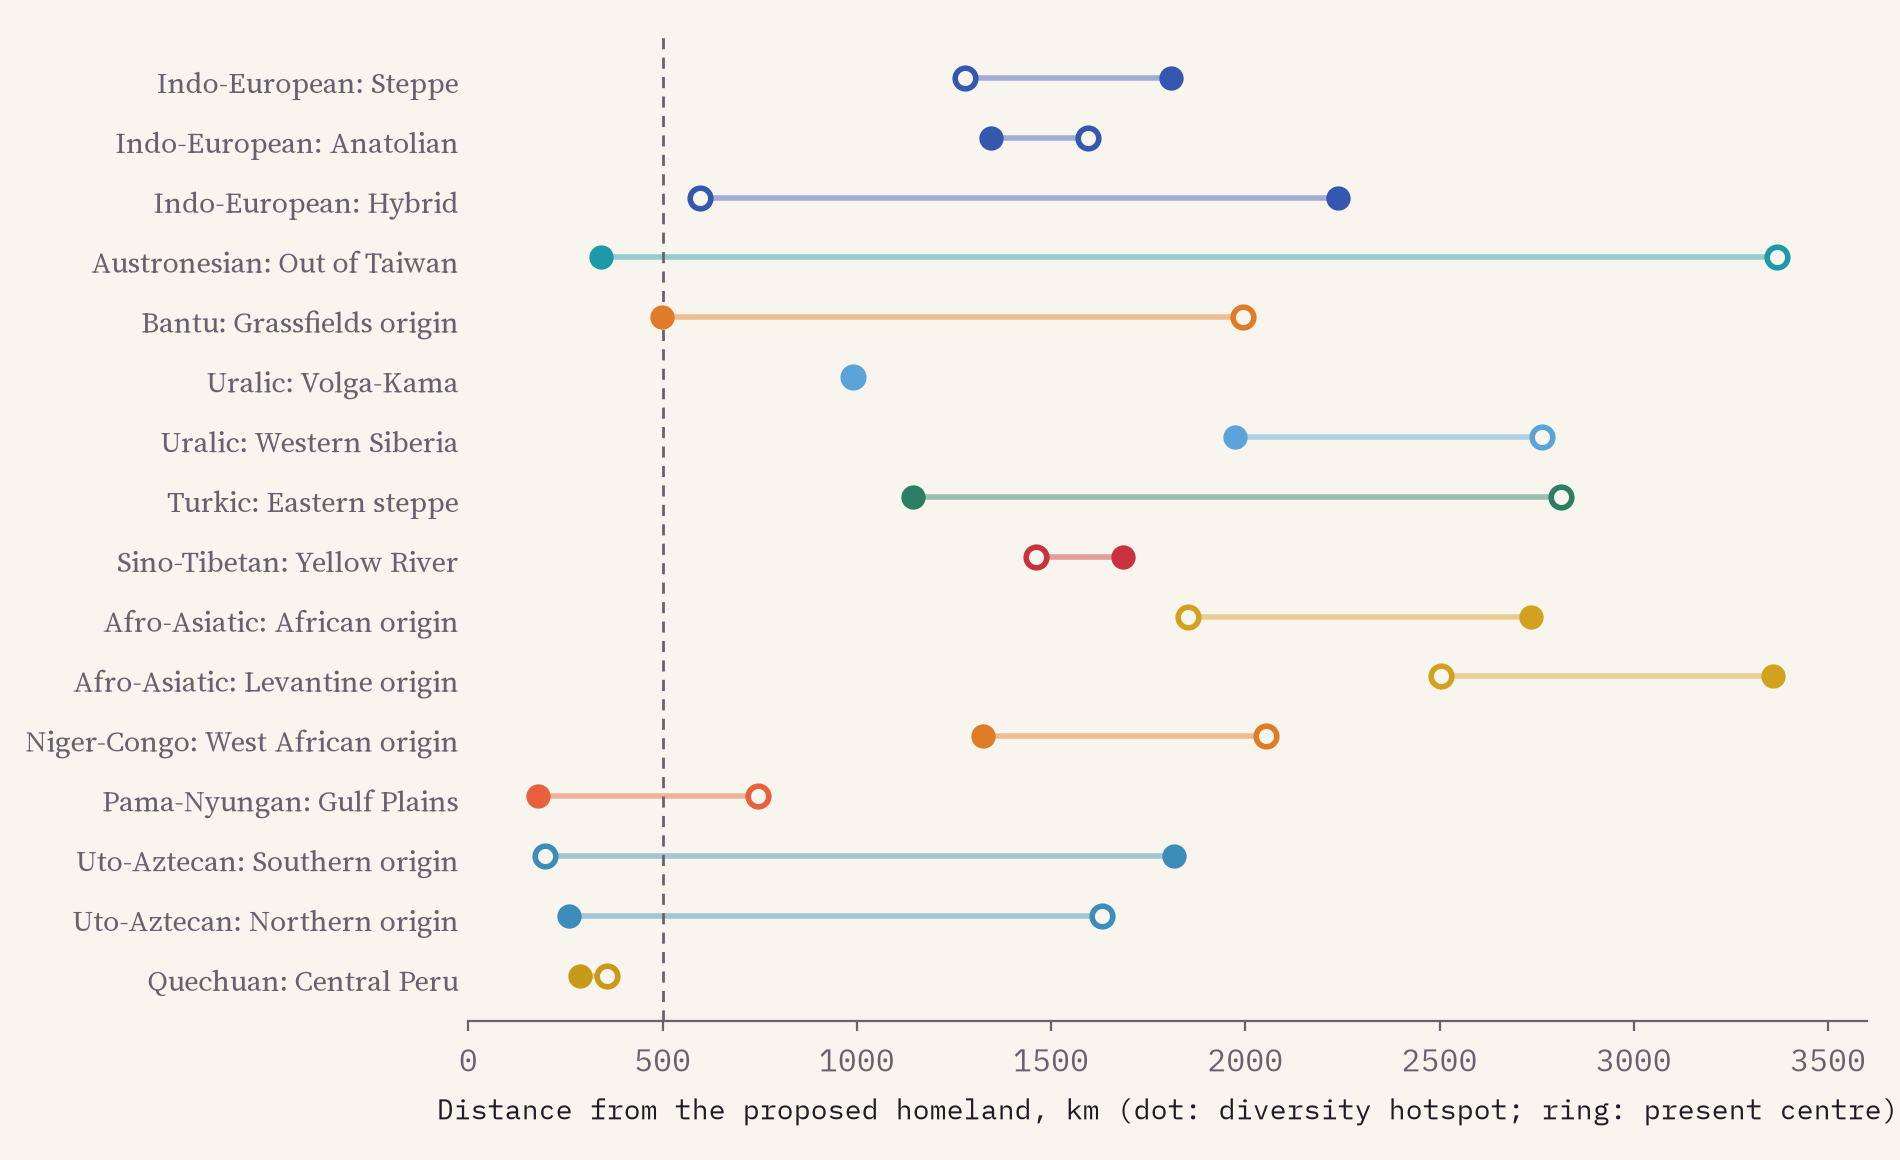
\includegraphics[width=.86\textwidth]{f_origins_dist.png}
\caption{Great-circle distance from each proposed homeland to the family's diversity hotspot (dot) and present centre (ring). Dashed line: 500 km.}\label{fig:dist}\end{figure}

For 5 of the 11 families the hotspot lies within 500 km of a proposed homeland (Austronesian, Bantu, Pama-Nyungan, Quechuan and the northern Uto-Aztecan proposal), whereas the present centre does so for only 2. The Austronesian hotspot is on Itbayat, between Taiwan and Luzon, 340 km from the Taiwan homeland; the family's present centre, pulled south-east by more than a thousand Malayo-Polynesian languages, is 3,368 km away. The Pama-Nyungan hotspot is 178 km from the Gulf Plains homeland of \citet{bouckaert2018}, the Quechuan hotspot 288 km from central Peru and the Bantu hotspot 497 km from the Grassfields (against 1,994 km for Bantu's present centre in the Congo basin).

The method fails where it would be expected to. The Indo-European hotspot falls near the Adriatic, where 6 of its 10 deep branches (Italic, Balto-Slavic, Albanian, Greek, Indo-Iranian through Romani, and Celtic) are found within 500 km. That reflects three thousand years of movement into the Balkans, not the family's beginning, and the hotspot is more than 1,000 km from all three proposals. The Sino-Tibetan hotspot falls in north-east India, where 15 of 19 deep branches meet; that is closer to the minority view of a south-western origin than to the Yellow River homeland of \citet{zhang2019} and \citet{sagart2019}, and it is a reminder that the hotspot measures where branches survive, which depends on later history. For Turkic and Afro-Asiatic, families shaped by large and recent expansions, neither computed point is near any proposed homeland.

\section{Discussion}
Glottolog makes it possible to describe the world's languages consistently from the level of the family down to the dialect. Three patterns stand out. First, linguistic history is deep and plural: more than four hundred lineages remain unconnected on present evidence, most of them small and many in the Americas and New Guinea. Second, diversity is concentrated in a tropical belt where small communities have lived alongside one another for a very long time, while most speakers belong to a handful of languages that spread with states and empires. Third, most of that diversity is at risk: a majority of languages are endangered, and in Australia and the Americas a large share are already gone.

On origins, a simple geographic heuristic recovers the accepted homelands of families whose spread is relatively recent and whose early branches were left behind in place, such as Austronesian and Bantu. It does not recover homelands where later migrations overlaid the early map, as for Indo-European and Turkic. That is consistent with the long-standing view that linguistic geography is evidence for, but not proof of, a homeland, and that ancient DNA and archaeology are needed to decide between hypotheses.

\section{Limitations}
First, the count of languages depends on where the line between language and dialect is drawn, and other catalogues count differently. Second, each language is a single point, usually the centre of its traditional area, so the map shows where languages come from rather than where their speakers now live; languages spoken across continents, such as English and Spanish, are one dot in Europe. Third, endangerment ratings are for whole languages, compiled from sources of different dates, and some will be out of date. Fourth, Wikidata speaker counts cover a minority of languages, favour larger ones, and mix first-language and total counts and years; the rule for choosing among them is a judgement. Fifth, country lists and coordinates in Glottolog are approximate, and grid counts depend on cell size and on coastlines. Sixth, the homeland hypotheses are typed in from the literature at the level of an approximate regional centre, and the computed hotspot and centre are heuristics sensitive to extinction, documentation and later migration. Finally, all data are from a single retrieval in 2026.

\section{Conclusion}
The world's 7,674 spoken languages belong to 421 lineages, are concentrated in a tropical belt, are mostly endangered and are spoken very unequally. The atlas lets readers explore the family tree, the geography of diversity and danger, and the competing hypotheses about where the great families began, with the evidence and its limits side by side.

\section*{Data and code availability}
The interactive atlas is at \url{https://maps.tristanhotham.com/language-origins/}. Data and code are at \url{https://github.com/Tristan-Hotham/language-origins} and archived with this paper at \url{https://doi.org/10.5281/zenodo.23844509}. Derived data are released under CC BY 4.0 (they include data from Glottolog, CC BY 4.0, and Wikidata, CC0), code under the MIT licence.

\section*{AI statement}
I wrote the text, with drafting and editing assistance from Claude (Anthropic), which also helped prepare the analysis code. I reviewed and checked all text and results.

\begin{thebibliography}{40}
\bibitem[Adelaar and Muysken(2004)]{adelaar2004} Adelaar, W. F. H. with Muysken, P. C. (2004) The Languages of the Andes. Cambridge University Press.
\bibitem[Anthony(2007)]{anthony2007} Anthony, D. W. (2007) The Horse, the Wheel, and Language: How Bronze-Age Riders from the Eurasian Steppes Shaped the Modern World. Princeton University Press.
\bibitem[Anthony and Ringe(2015)]{anthony2015} Anthony, D. W. and Ringe, D. (2015) The Indo-European homeland from linguistic and archaeological perspectives. Annual Review of Linguistics 1, 199 to 219.
\bibitem[Blust(1999)]{blust1999} Blust, R. (1999) Subgrouping, circularity and extinction: some issues in Austronesian comparative linguistics. In Zeitoun, E. and Li, P. J.-K. (eds) Selected Papers from the Eighth International Conference on Austronesian Linguistics. Academia Sinica, 31 to 94.
\bibitem[Bouckaert et al.(2018)]{bouckaert2018} Bouckaert, R. R., Bowern, C. and Atkinson, Q. D. (2018) The origin and expansion of Pama-Nyungan languages across Australia. Nature Ecology and Evolution 2, 741 to 749.
\bibitem[Bouckaert et al.(2012)]{bouckaert2012} Bouckaert, R. et al. (2012) Mapping the origins and expansion of the Indo-European language family. Science 337, 957 to 960.
\bibitem[Ehret(1995)]{ehret1995} Ehret, C. (1995) Reconstructing Proto-Afroasiatic (Proto-Afrasian): Vowels, Tone, Consonants, and Vocabulary. University of California Press.
\bibitem[Ehret et al.(2004)]{ehret2004} Ehret, C., Keita, S. O. Y. and Newman, P. (2004) The origins of Afroasiatic. Science 306, 1680 to 1681.
\bibitem[Fowler(1983)]{fowler1983} Fowler, C. S. (1983) Some lexical clues to Uto-Aztecan prehistory. International Journal of American Linguistics 49, 224 to 257.
\bibitem[Golden(1992)]{golden1992} Golden, P. B. (1992) An Introduction to the History of the Turkic Peoples. Harrassowitz.
\bibitem[Gray et al.(2009)]{gray2009} Gray, R. D., Drummond, A. J. and Greenhill, S. J. (2009) Language phylogenies reveal expansion pulses and pauses in Pacific settlement. Science 323, 479 to 483.
\bibitem[Grollemund et al.(2015)]{grollemund2015} Grollemund, R. et al. (2015) Bantu expansion shows that habitat alters the route and pace of human dispersals. Proceedings of the National Academy of Sciences 112, 13296 to 13301.
\bibitem[Grünthal et al.(2022)]{grunthal2022} Grünthal, R., Heyd, V., Holopainen, S., Janhunen, J., Khanina, O., Miestamo, M., Nichols, J., Saarikivi, J. and Sinnemäki, K. (2022) Drastic demographic events triggered the Uralic spread. Diachronica 39(4), 490 to 524.
\bibitem[Güldemann(2018)]{guldemann2018} Güldemann, T. (2018) Historical linguistics and genealogical language classification in Africa. In Güldemann, T. (ed.) The Languages and Linguistics of Africa. De Gruyter Mouton, 58 to 444.
\bibitem[Haak et al.(2015)]{haak2015} Haak, W. et al. (2015) Massive migration from the steppe was a source for Indo-European languages in Europe. Nature 522, 207 to 211.
\bibitem[Hammarström et al.(2025)]{glottolog} Hammarström, H., Forkel, R., Haspelmath, M. and Bank, S. (2025) Glottolog 5.2.1. Leipzig: Max Planck Institute for Evolutionary Anthropology. CLDF release, CC BY 4.0. \url{https://glottolog.org}
\bibitem[Heggarty et al.(2023)]{heggarty2023} Heggarty, P. et al. (2023) Language trees with sampled ancestors support a hybrid model for the origin of Indo-European languages. Science 381, eabg0818.
\bibitem[Hill(2001)]{hill2001} Hill, J. H. (2001) Proto-Uto-Aztecan: a community of cultivators in central Mexico? American Anthropologist 103, 913 to 934.
\bibitem[Honkola et al.(2013)]{honkola2013} Honkola, T. et al. (2013) Cultural and climatic changes shape the evolutionary history of the Uralic languages. Journal of Evolutionary Biology 26, 1244 to 1253.
\bibitem[Janhunen(2009)]{janhunen2009} Janhunen, J. (2009) Proto-Uralic: what, where, and when? In Ylikoski, J. (ed.) The Quasquicentennial of the Finno-Ugrian Society. Mémoires de la Société Finno-Ougrienne 258, 57 to 78.
\bibitem[Militarev(2002)]{militarev2002} Militarev, A. (2002) The prehistory of a dispersal: the Proto-Afrasian (Afroasiatic) farming lexicon. In Bellwood, P. and Renfrew, C. (eds) Examining the Farming/Language Dispersal Hypothesis. McDonald Institute for Archaeological Research, 135 to 150.
\bibitem[Natural Earth(2026)]{naturalearth} Natural Earth (2026) Admin 0 countries, land, admin 1 states and provinces, populated places. Public domain. \url{https://www.naturalearthdata.com/}
\bibitem[Renfrew(1987)]{renfrew1987} Renfrew, C. (1987) Archaeology and Language: The Puzzle of Indo-European Origins. Jonathan Cape.
\bibitem[Sagart et al.(2019)]{sagart2019} Sagart, L. et al. (2019) Dated language phylogenies shed light on the ancestry of Sino-Tibetan. Proceedings of the National Academy of Sciences 116, 10317 to 10322.
\bibitem[Sapir(1916)]{sapir1916} Sapir, E. (1916) Time Perspective in Aboriginal American Culture: A Study in Method. Geological Survey of Canada, Memoir 90.
\bibitem[Savelyev and Robbeets(2020)]{savelyev2020} Savelyev, A. and Robbeets, M. (2020) Bayesian phylolinguistics infers the internal structure and the time-depth of the Turkic language family. Journal of Language Evolution 5(1), 39-53. doi:10.1093/jole/lzz010
\bibitem[Šavrič et al.(2019)]{equalearth} Šavrič, B., Patterson, T. and Jenny, B. (2019) The Equal Earth map projection. \emph{International Journal of Geographical Information Science} 33(3), 454 to 465.
\bibitem[Torero(1964)]{torero1964} Torero, A. (1964) Los dialectos quechuas. Anales Científicos de la Universidad Agraria 2, 446 to 478.
\bibitem[Vansina(1995)]{vansina1995} Vansina, J. (1995) New linguistic evidence and 'the Bantu expansion'. Journal of African History 36, 173 to 195.
\bibitem[Vrandečić and Krötzsch(2014)]{wikidata} Vrandečić, D. and Krötzsch, M. (2014) Wikidata: a free collaborative knowledgebase. \emph{Communications of the ACM} 57(10), 78 to 85. Data CC0, \url{https://www.wikidata.org/}
\bibitem[Williamson and Blench(2000)]{williamson2000} Williamson, K. and Blench, R. (2000) Niger-Congo. In Heine, B. and Nurse, D. (eds) African Languages: An Introduction. Cambridge University Press, 11 to 42.
\bibitem[Zhang et al.(2019)]{zhang2019} Zhang, M., Yan, S., Pan, W. and Jin, L. (2019) Phylogenetic evidence for Sino-Tibetan origin in northern China in the Late Neolithic. Nature 569, 112 to 115.
\end{thebibliography}
\end{document}
